% -*- coding: utf-8 -*-
%-------------------------designed by zcf--------------
\documentclass[UTF8,a4paper,10pt]{ctexart}
\usepackage[left=3.17cm, right=3.17cm, top=2.74cm, bottom=2.74cm]{geometry}
\usepackage{amsmath}
\usepackage{graphicx,subfig}
\usepackage{float}
\usepackage{cite}
\usepackage{caption}
\usepackage{enumerate}
\usepackage{booktabs} %表格
\usepackage{multirow}
\newcommand{\tabincell}[2]{\begin{tabular}{@{}#1@{}}#2\end{tabular}}  %表格强制换行
%-------------------------字体设置--------------
% \usepackage{times} 
\usepackage{ctex}
\setCJKmainfont[ItalicFont=Noto Sans CJK SC Bold, BoldFont=Noto Serif CJK SC Black]{Noto Serif CJK SC}
\newcommand{\yihao}{\fontsize{26pt}{36pt}\selectfont}           % 一号, 1.4 倍行距
\newcommand{\erhao}{\fontsize{22pt}{28pt}\selectfont}          % 二号, 1.25倍行距
\newcommand{\xiaoer}{\fontsize{18pt}{18pt}\selectfont}          % 小二, 单倍行距
\newcommand{\sanhao}{\fontsize{16pt}{24pt}\selectfont}  %三号字
\newcommand{\xiaosan}{\fontsize{15pt}{22pt}\selectfont}        % 小三, 1.5倍行距
\newcommand{\sihao}{\fontsize{14pt}{21pt}\selectfont}            % 四号, 1.5 倍行距
\newcommand{\banxiaosi}{\fontsize{13pt}{19.5pt}\selectfont}    % 半小四, 1.5倍行距
\newcommand{\xiaosi}{\fontsize{12pt}{18pt}\selectfont}            % 小四, 1.5倍行距
\newcommand{\dawuhao}{\fontsize{11pt}{11pt}\selectfont}       % 大五号, 单倍行距
\newcommand{\wuhao}{\fontsize{10.5pt}{15.75pt}\selectfont}    % 五号, 单倍行距
%-------------------------章节名----------------
\usepackage{ctexcap} 
\CTEXsetup[name={,、},number={ \chinese{section}}]{section}
\CTEXsetup[name={(,)},number={\chinese{subsection}}]{subsection}
\CTEXsetup[name={,.},number={\arabic{subsubsection}}]{subsubsection}
%-------------------------页眉页脚--------------
\usepackage{fancyhdr}
\pagestyle{fancy}
\lhead{\kaishu \leftmark}
% \chead{}
\rhead{\kaishu 编译原理实验报告}%加粗\bfseries 
\lfoot{}
\cfoot{\thepage}
\rfoot{}
\renewcommand{\headrulewidth}{0.1pt}  
\renewcommand{\footrulewidth}{0pt}%去掉横线
\newcommand{\HRule}{\rule{\linewidth}{0.5mm}}%标题横线
\newcommand{\HRulegrossa}{\rule{\linewidth}{1.2mm}}
%-----------------------伪代码------------------
\usepackage{algorithm}  
\usepackage{algorithmicx}  
\usepackage{algpseudocode}  
\floatname{algorithm}{Algorithm}  
\renewcommand{\algorithmicrequire}{\textbf{Input:}}  
\renewcommand{\algorithmicensure}{\textbf{Output:}} 
\usepackage{lipsum}  
\makeatletter
\newenvironment{breakablealgorithm}
  {% \begin{breakablealgorithm}
  \begin{center}
     \refstepcounter{algorithm}% New algorithm
     \hrule height.8pt depth0pt \kern2pt% \@fs@pre for \@fs@ruled
     \renewcommand{\caption}[2][\relax]{% Make a new \caption
      {\raggedright\textbf{\ALG@name~\thealgorithm} ##2\par}%
      \ifx\relax##1\relax % #1 is \relax
         \addcontentsline{loa}{algorithm}{\protect\numberline{\thealgorithm}##2}%
      \else % #1 is not \relax
         \addcontentsline{loa}{algorithm}{\protect\numberline{\thealgorithm}##1}%
      \fi
      \kern2pt\hrule\kern2pt
     }
  }{% \end{breakablealgorithm}
     \kern2pt\hrule\relax% \@fs@post for \@fs@ruled
  \end{center}
  }
\makeatother
%------------------------代码-------------------
\usepackage{xcolor} 
\usepackage{listings} 
\lstset{ 
breaklines,%自动换行
basicstyle=\small,
escapeinside=``,
keywordstyle=\color{ blue!70} \bfseries,
commentstyle=\color{red!50!green!50!blue!50},% 
stringstyle=\ttfamily,% 
extendedchars=false,% 
linewidth=\textwidth,% 
numbers=left,% 
numberstyle=\tiny \color{blue!50},% 
frame=trbl% 
rulesepcolor= \color{ red!20!green!20!blue!20} 
}
%------------超链接----------
\usepackage[colorlinks,linkcolor=black,anchorcolor=blue]{hyperref}
%------------------------TODO-------------------
\usepackage{enumitem,amssymb}
\newlist{todolist}{itemize}{2}
\setlist[todolist]{label=$\square$}
% for check symbol 
\usepackage{pifont}
\newcommand{\cmark}{\ding{51}}%
\newcommand{\xmark}{\ding{55}}%
\newcommand{\done}{\rlap{$\square$}{\raisebox{2pt}{\large\hspace{1pt}\cmark}}\hspace{-2.5pt}}
\newcommand{\wontfix}{\rlap{$\square$}{\large\hspace{1pt}\xmark}}
%------------------------水印-------------------
\usepackage{tikz}
\usepackage{xcolor}
\usepackage{eso-pic}

\newcommand{\watermark}[3]{\AddToShipoutPictureBG{
\parbox[b][\paperheight]{\paperwidth}{
\vfill%
\centering%
\tikz[remember picture, overlay]%
  \node [rotate = #1, scale = #2] at (current page.center)%
    {\textcolor{gray!80!cyan!30!magenta!30}{#3}};
\vfill}}}



%———————————————————————————————————————————正文———————————————————————————————————————————————
%----------------------------------------------
\begin{document}
\begin{titlepage}
    \begin{center}
    \includegraphics[width=0.8\textwidth]{NKU.png}\\[1cm]    
    \textsc{\Huge \kaishu{\textbf{南\ \ \ \ \ \ 开\ \ \ \ \ \ 大\ \ \ \ \ \ 学}} }\\[0.9cm]
    \textsc{\huge \kaishu{\textbf{网\ \ 络\ \ 空\ \ 间\ \ 安\ \ 全\ \ 学\ \ 院}}}\\[0.5cm]
    \textsc{\Large \textbf{编译原理实验报告}}\\[0.8cm]
    \HRule \\[0.9cm]
    { \LARGE \bfseries 实现SysY编译器}\\[0.4cm]
    \HRule \\[2.0cm]
    \centering
    \textsc{\LARGE \kaishu{周延霖\ 2013921}}\\[0.5cm]
    \textsc{\LARGE \kaishu{年级\ :\ 2020级}}\\[0.5cm]
    \textsc{\LARGE \kaishu{专业\ :\ 信息安全}}\\[0.5cm]
    \textsc{\LARGE \kaishu{指导教师\ :\ 王刚}}\\[0.5cm]
    \vfill
    {\Large \today}
    \end{center}
\end{titlepage}
%-------------摘------要--------------
\newpage
\thispagestyle{empty}
\renewcommand{\abstractname}{\kaishu \sihao \textbf{摘要}}
    \begin{abstract}
        在本学期编译原理课程中完整实现了一个SysY语言的编译器,在本篇文章中将对其从开始的词法分析、语法分析到后来的中间代码、目标代码生成进行逐一介绍,并在最后对完成所有任务后的优化进行简介。
        \noindent  %顶格
        \textbf{\\\ 关键字:}\textbf{SysY语言、编译原理、指令翻译} \\\ \\\
    \end{abstract}
%----------------------------------------------------------------
\tableofcontents
%----------------------------------------------------------------
\newpage
\watermark{60}{10}{NKU}
\setcounter{page}{1}




%----------------------------------------------------------------





%----------------------------------------------------------------
% 引言开始
\newpage

\section{引言}
编译原理课程兼有很强的理论性和实践性,是计算机专业的一门非常重要的专业基础课程,在系统软件中占有十分重要的地位。编译原理课程设计是本课程重要的综合实践教学环节,是对平时实验的一个补充。通过编译器相关子系统的设计,使我们能够更好地掌握编译原理的基本理论和编译程序构造的慕木方法和技巧,融会贯通本课程所学专业理讼知识:培养学生独立分析问题、解决问题的能力,以及系统软件设计的能力:培养学生的创新能力及团队协作精神。


一个编译器所进行的工作一般可以划分为五个阶段:词法分析、语法分析、语义分析和中间代码产生、中间代码的优化、目标代码生成。

首先是词法分析,针对词法分析,我们设计了一个可以识别绝大部分标准SysY语言支特的词法符号,该词法分析器可以过滤空格、Tab和回车,并且支持注释功能,即过滤掉注释符号后面的代码。词法分析器在识别到一个单词后,将该单词记录下来,如果是数据,则会在符号表的相应位置记录它的值,如果是标识符,则会先在符号表上进行查询,若没有则将其记录到符号表上,并将相应TOKEN 的指针指向表中该位置。

接下来进行语法分析,在语法分析部分,会对所编写的代码的语法进行检验,看是否合乎我们所设定的语法规则,所设计的文法支特了函数、函数类型声明、变量类型声明、变量定义、表达式语句、if条件语句和while循环语句等。在表达式语句方面,我们设计了支持所有算术运算、关系运算、逻辑运算和位运算功能的语法结构,并且语法上支持数组。

在类型检查(语义分析)和中间代码产生的阶段。我们在语法分析程序的相应部分加上了语义动作。在语义分析部分主要是对语法分析器的输出进行检查,并提供相应的错误,这是对程序员友好的。在中间代码部分根据正确的程序进行基本块的构建,流图的构建,并最终遍历语法树,输出中间代码。

最后一个阶段是目标代码生成。在这一步骤需要将中间代码提供的输出转换成真正的可以在环境中运行的汇编代码,需要分配真实存在的物理寄存器,在这一步骤中,我们完成了所有的提高要求,并对寄存器分配进行优化,最终通过了所有的151个测试样例。

本次的所有代码已经上传于gitlab,链接如下:\\
\href{git@gitlab.eduxiji.net:nku-hlast/lab2.git}{SSH: git@gitlab.eduxiji.net:nku-hlast/lab2.git}\\
\href{https://gitlab.eduxiji.net/nku-hlast/lab2.git}{HTTP:  https://gitlab.eduxiji.net/nku-hlast/lab2.git}

% 引言结束
%----------------------------------------------------------------









%----------------------------------------------------------------
% 词法分析开始
\newpage

\section{词法分析}
\subsection{模块设计}
\subsubsection{功能简述}
在词法分析的实验中,我们利用\fbox{Flex}工具实现了词法分析器,识别输入的\fbox{SysY}语言程序中的所有单词,并将其转化为单词流,输出为每一个文法单元的类别、词素,以及必要的属性。

例如,对于 NUMBER 会有属于它的“数值”属性;对于 ID 会有它在符号表的“序号”,
有些标识符会有相同的“序号”。

在此次实验中,我们已经设计了符号表,但不过只是实现了一些简单的功能,比如保存词素等简单内容,但是符号表的数据结构,搜索算法,词素的保存,保留字的处理等问题将放到后续实验中进行。

\subsubsection{设计目标}
首先,Flex的词法规则主要由3部分组成,部分之间使用\fbox{\%\%}分隔

\begin{itemize}
  \item 第一部分:由选项和声明组成。\%\{ \%\}围住的部分会被原封不动的复制到Flex生成的词法分析器代码靠近前面的地方。
  \item 第二部分:由一系列的匹配规则(Pattern)和动作(Action)组成,每行一个匹配规则和一个动作。匹配采用了正则表达式,动作是纯C代码编写的,放在{ }里面,可以有多行代码。动作描述了匹配到规则后执行的操作,上面的例子的动作是打印提示信息。
  \item 第三部分:是C语言代码,会直接被复制到生成的词法生成器代码中。一般都是main程序,是词法分析器的入口。
\end{itemize}

在本次实验中,主要利用已有框架,在第二部分完成对8进制、16进制等整型的翻译,并识别相应的符号将其存入到符号表中,最后通过分析.sy文件将其中的重要信息输出。



\subsection{个人贡献}
\subsubsection{负责任务}
由于本次实验整体上不复杂,所以我们首先分别对自己的词法分析器进行实现,然后进行整合,每个部分选出实现更简单完成较好的代码,最后提交到gitlab上。

主要任务如下:
\begin{itemize}
  \item 补全缺失的正则定义
  \item 参考 “int” 的规则,完成其他大部分终结符的规则定义
  \item 完成八进制数字、十六进制数字的规则定义,将其保存为十进制输出
  \item 完成标识符相关规则定义以及符号表
  \item 完成注释的正则定义和规则定义
  \item 完成对程序的输出
\end{itemize}


\subsubsection{任务实现}
\paragraph{正则定义}
对于正则定义部分需要完成对例如如八进制数字、十六进制数字、行注释等内容的补全,补全后的正则定义部分如下:
\begin{lstlisting}[title = 词法分析部分的正则定义]
HEX (0x[1-9|A-F|a-f][0-9|A-F|a-f]*|0x0)
OCT (0[1-7][0-7]*|00)
DECIMIAL ([1-9][0-9]*|0)
ID [[:alpha:]_][[:alpha:][:digit:]_]*
char ('.')
EOL (\r\n|\n|\r)
WHITE [\t ]
linecomment \/\/.*
commentbegin "/*"
commentelement .|\n
commentend "*/"

%x BLOCKCOMMENT
\end{lstlisting}
如上所示,仿照10进制对8进制和16进制进行补充定义,比如像8进制当识别到0开始的数字串的时候就可以确定是8进制串了,并加上了识别符号(由字母、数字和符号组成)以及注释等正则定义,在这之中,声明部分的\%x声明了一个新的起始状态,而在之后的规则使用中加入< 状态名 >的表明该规则只在当前状态下生效。

\paragraph{终结符定义}
对于大部分的终结符,其实“int”已经写的非常明确了,只需要将int改个名字,其余部分照做即可,比如说void的定义如下:
\begin{lstlisting}[title = 仿照int定义void]
"void" {
    #ifdef ONLY_FOR_LEX
        char content[100];
        sprintf(content,"%-10s","VOID");
        AppendChar(content,"void");
        // strcpy(content,"VOID\tvoid");
        AddLineNo(content,yylineno);
        AddOffset(content,offset);
        offset += 4;
        DEBUG_FOR_LAB4(content);
    #else
        return VOID;
    #endif 
}
\end{lstlisting}

可以看到只需将相应位置改名即可,但要注意的是return后面的返回值是需要为语法分析做铺垫的,所以此次命名的返回值在将来语法分析器部分也是要用相同的名字,所以按照关键词来设计就不会造成冲突。

\paragraph{进制转换}
对于进制转换来说8进制和16进制是相似的,所以在这里解释一下16进制的转换,代码如下:

\begin{lstlisting}[title = 16进制转换]
{HEX} {
    #ifdef ONLY_FOR_LEX
        string a  = yytext;
        int len = a.length() - 2;
        int all = 0;
        for(int i = 0; i < len; i++)
        {
            int temp1 = (pow(16, (len - i - 1)));
            int temp2;
            if(a[i + 2] >= '0' && a[i + 2] <= '9'){
                temp2 = (a[i + 2] - '0');
            }
            else if(a[i + 2] >= 'A' && a[i + 2] <= 'F'){
                temp2 = a[i + 2] - 'A' + 10;
            }
            else if(a[i + 2] >= 'a' && a[i + 2] <= 'f'){
                temp2 = a[i + 2] - 'a' + 10;
            }
            all = all + temp1 * temp2;         
        }
        string temp = "HEX\t" + to_string(all) + "(DEC)" + "\tlinecount:" + to_string(yylineno);
        DEBUG_FOR_LAB4(temp);
    #else 
        return HEX;
    #endif
}
\end{lstlisting}
逻辑思路是循环输入字符的每一位,根据时字符还是数字来对其进行对应的加减操作,并乘以当前所在的位置的16的次方,然后将其加到总和中,最后返回即可。
\paragraph{标识符}
\subparagraph{符号表}
对于符号表来说本次实现的较为简单,声明一个结构体,存储它的值以及作用域,然后定义一个此结构体的容器,相当于一个简易的符号表。
\subparagraph{作用域}
由于每个符号都有一定的作用域,在不同的作用域中的符号可使用相同的名字,在同一个作用域就不能出现这种情况,也方便之后对于重定义的类型检查的判断,在这里判断作用域的方法主要是根据大括号:
\begin{lstlisting}[title = 作用域的判断]
"{" {
    #ifdef ONLY_FOR_LEX
        global_count_of_id++;
        a.push_back(global_count_of_id);
        //cout << "{" << a.back() << endl;
        leftNum++;
        string temp = "LBRACE\t{\tlinecount:" + to_string(yylineno);
        DEBUG_FOR_LAB4(temp);
    #else
        return LBRACE;
    #endif
}
"}" {
    #ifdef ONLY_FOR_LEX
        a.pop_back();
        //cout << "}" << a.back() << endl;
        rightNum++;
        string temp = "RBRACE\t}\tlinecount:" + to_string(yylineno);
        DEBUG_FOR_LAB4(temp);
    #else
        return RBRACE;
    #endif
}
\end{lstlisting}
事先定义一个全局的变量\fbox{global\_count\_of\_id},在每次出现左大括号时将其加一并加入容器,在每次出现右大括号是将其弹出,这样在任何时候出现标识符都可以知道当前对应的数字,来区分不同的作用域。
\subparagraph{定义}
当作用域和符号表实现之后,对于标识符的实现就变得简单了,具体如下:
\begin{lstlisting}[title = 标识符的实现]
{ID} {
    #ifdef ONLY_FOR_LEX
        string m = yytext;
        //cout << yytext << ":" << a.size() << endl;
        int idnum = 0;
        bool flag = 0;
        for(int i = 0; i < id_count; i++)
        {
            if(table[i].name_of_id == yytext && table[i].global_count_of_id == a.back())
            {
                idnum = i + 1;
                flag = 1;
                break;
            }
        }
        if(flag == 0)
        {
            table[id_count].name_of_id = yytext;
            if(a.size() != 0){
                table[id_count].global_count_of_id = a.back();
            }
            id_count++;
            idnum = id_count;
        }
        string temp = "ID\t" + m + "\tlinecount:" + to_string(yylineno) + "\tIDcount:" + to_string(idnum);
        DEBUG_FOR_LAB4(temp);
    #else 
        return ID;
    #endif
}
\end{lstlisting}
在每次出现标识符时在符号表中查找,如果有就直接输出,如果没有就根据当前的作用域和它的值将其加入符号表中即可
\paragraph{注释}
实现多行注释的时候,重点是状态的切换和换行的处理,在这里解释一下对结束注释的处理,其余类似:
\begin{lstlisting}[title = 结束注释的处理]
<BLOCKCOMMENT>{commentend} {
    #ifdef ONLY_FOR_LEX
        string a = yytext;
        if(a.find("\n") != a.npos)
        {
            yylineno++;
            a.replace(a.find("\n"),1,"");
        }
        string temp = "commentend\t" + a + "\tlinecount:" + to_string(yylineno);
        DEBUG_FOR_LAB4(temp);
        BEGIN INITIAL;
    #else 
        return commentend;
    #endif
}
\end{lstlisting}
当出现换行时,需要将全局变量yylineno进行加1操作,并在结束完成后切换到初始状态。

\paragraph{程序输出}
程序的输出其实主要是看是否成功捕获到相应的关系,所以将每个识别出来的变量赋予一个字符串,然后调用输出函数即可完成。



\subsubsection{结果展示}

词法分析部分手写的样例代码如下:

\begin{lstlisting}[title = 词法分析样例代码, language = c++]
// i am a function: this function has many syntax errors.

int f(){
	int a;
	a = 0;
	while(a<10){
		a = a * 2345;
	}
	return a;
}

int main(){
	int _testid;
	_testid = 0;
	if(_testid==0){
		int _testid;
		int _testid2;
		_testid1=_testid1+1;
	}
	/*
		Comment lines;
	*/
	{
		int a;
	}
	{
		int a;
	}
	int b;
	return 0;
}

/*
	Comment lines.
*/
\end{lstlisting}

词法分析所对应的元素分析如下:

\begin{lstlisting}[title = 词法分析结果]
[DEBUG LAB4]: 	linecomment	// i am a function: this function has many syntax errors.	linecount:1
[DEBUG LAB4]: 	INT	int	linecount:3
[DEBUG LAB4]: 	ID	f	linecount:3	IDcount:1
[DEBUG LAB4]: 	LPAREN	(	linecount:3
[DEBUG LAB4]: 	RPAREN	)	linecount:3
[DEBUG LAB4]: 	LBRACE	{	linecount:3
[DEBUG LAB4]: 	INT	int	linecount:4
[DEBUG LAB4]: 	ID	a	linecount:4	IDcount:2
[DEBUG LAB4]: 	SEMICOLON	;	linecount:4
[DEBUG LAB4]: 	ID	a	linecount:5	IDcount:2
[DEBUG LAB4]: 	ASSIGN	=	linecount:5
[DEBUG LAB4]: 	DECIMIAL	0	linecount:5
[DEBUG LAB4]: 	SEMICOLON	;	linecount:5
[DEBUG LAB4]: 	WHILE	while	linecount:6
[DEBUG LAB4]: 	LPAREN	(	linecount:6
[DEBUG LAB4]: 	ID	a	linecount:6	IDcount:2
[DEBUG LAB4]: 	LESS	<	linecount:6
[DEBUG LAB4]: 	DECIMIAL	10	linecount:6
[DEBUG LAB4]: 	RPAREN	)	linecount:6
[DEBUG LAB4]: 	LBRACE	{	linecount:6
[DEBUG LAB4]: 	ID	a	linecount:7	IDcount:3
[DEBUG LAB4]: 	ASSIGN	=	linecount:7
[DEBUG LAB4]: 	ID	a	linecount:7	IDcount:3
[DEBUG LAB4]: 	STAR	*	linecount:7
[DEBUG LAB4]: 	DECIMIAL	2345	linecount:7
[DEBUG LAB4]: 	SEMICOLON	;	linecount:7
[DEBUG LAB4]: 	RBRACE	}	linecount:8
[DEBUG LAB4]: 	RETURN	return	linecount:9
[DEBUG LAB4]: 	ID	a	linecount:9	IDcount:2
[DEBUG LAB4]: 	SEMICOLON	;	linecount:9
[DEBUG LAB4]: 	RBRACE	}	linecount:10
[DEBUG LAB4]: 	INT	int	linecount:12
[DEBUG LAB4]: 	ID	main	linecount:12	IDcount:4
[DEBUG LAB4]: 	LPAREN	(	linecount:12
[DEBUG LAB4]: 	RPAREN	)	linecount:12
[DEBUG LAB4]: 	LBRACE	{	linecount:12
[DEBUG LAB4]: 	INT	int	linecount:13
[DEBUG LAB4]: 	ID	_testid	linecount:13	IDcount:5
[DEBUG LAB4]: 	SEMICOLON	;	linecount:13
[DEBUG LAB4]: 	ID	_testid	linecount:14	IDcount:5
[DEBUG LAB4]: 	ASSIGN	=	linecount:14
[DEBUG LAB4]: 	DECIMIAL	0	linecount:14
[DEBUG LAB4]: 	SEMICOLON	;	linecount:14
[DEBUG LAB4]: 	IF	if	linecount:15
[DEBUG LAB4]: 	LPAREN	(	linecount:15
[DEBUG LAB4]: 	ID	_testid	linecount:15	IDcount:5
[DEBUG LAB4]: 	EQUAL	==	linecount:15
[DEBUG LAB4]: 	DECIMIAL	0	linecount:15
[DEBUG LAB4]: 	RPAREN	)	linecount:15
[DEBUG LAB4]: 	LBRACE	{	linecount:15
[DEBUG LAB4]: 	INT	int	linecount:16
[DEBUG LAB4]: 	ID	_testid	linecount:16	IDcount:6
[DEBUG LAB4]: 	SEMICOLON	;	linecount:16
[DEBUG LAB4]: 	INT	int	linecount:17
[DEBUG LAB4]: 	ID	_testid2	linecount:17	IDcount:7
[DEBUG LAB4]: 	SEMICOLON	;	linecount:17
[DEBUG LAB4]: 	ID	_testid1	linecount:18	IDcount:8
[DEBUG LAB4]: 	ASSIGN	=	linecount:18
[DEBUG LAB4]: 	ID	_testid1	linecount:18	IDcount:8
[DEBUG LAB4]: 	ADD	+	linecount:18
[DEBUG LAB4]: 	DECIMIAL	1	linecount:18
[DEBUG LAB4]: 	SEMICOLON	;	linecount:18
[DEBUG LAB4]: 	RBRACE	}	linecount:19
[DEBUG LAB4]: 	commentbegin	/*	linecount:20
[DEBUG LAB4]: 	commentelement		linecount:21
[DEBUG LAB4]: 	commentelement			linecount:21
[DEBUG LAB4]: 	commentelement			linecount:21
[DEBUG LAB4]: 	commentelement	C	linecount:21
[DEBUG LAB4]: 	commentelement	o	linecount:21
[DEBUG LAB4]: 	commentelement	m	linecount:21
[DEBUG LAB4]: 	commentelement	m	linecount:21
[DEBUG LAB4]: 	commentelement	e	linecount:21
[DEBUG LAB4]: 	commentelement	n	linecount:21
[DEBUG LAB4]: 	commentelement	t	linecount:21
[DEBUG LAB4]: 	commentelement	 	linecount:21
[DEBUG LAB4]: 	commentelement	l	linecount:21
[DEBUG LAB4]: 	commentelement	i	linecount:21
[DEBUG LAB4]: 	commentelement	n	linecount:21
[DEBUG LAB4]: 	commentelement	e	linecount:21
[DEBUG LAB4]: 	commentelement	s	linecount:21
[DEBUG LAB4]: 	commentelement	;	linecount:21
[DEBUG LAB4]: 	commentelement		linecount:22
[DEBUG LAB4]: 	commentelement			linecount:22
[DEBUG LAB4]: 	commentend	*/	linecount:22
[DEBUG LAB4]: 	LBRACE	{	linecount:23
[DEBUG LAB4]: 	INT	int	linecount:24
[DEBUG LAB4]: 	ID	a	linecount:24	IDcount:9
[DEBUG LAB4]: 	SEMICOLON	;	linecount:24
[DEBUG LAB4]: 	RBRACE	}	linecount:25
[DEBUG LAB4]: 	LBRACE	{	linecount:26
[DEBUG LAB4]: 	INT	int	linecount:27
[DEBUG LAB4]: 	ID	a	linecount:27	IDcount:10
[DEBUG LAB4]: 	SEMICOLON	;	linecount:27
[DEBUG LAB4]: 	RBRACE	}	linecount:28
[DEBUG LAB4]: 	INT	int	linecount:29
[DEBUG LAB4]: 	ID	b	linecount:29	IDcount:11
[DEBUG LAB4]: 	SEMICOLON	;	linecount:29
[DEBUG LAB4]: 	RETURN	return	linecount:30
[DEBUG LAB4]: 	DECIMIAL	0	linecount:30
[DEBUG LAB4]: 	SEMICOLON	;	linecount:30
[DEBUG LAB4]: 	RBRACE	}	linecount:31
[DEBUG LAB4]: 	commentbegin	/*	linecount:33
[DEBUG LAB4]: 	commentelement		linecount:34
[DEBUG LAB4]: 	commentelement			linecount:34
[DEBUG LAB4]: 	commentelement	C	linecount:34
[DEBUG LAB4]: 	commentelement	o	linecount:34
[DEBUG LAB4]: 	commentelement	m	linecount:34
[DEBUG LAB4]: 	commentelement	m	linecount:34
[DEBUG LAB4]: 	commentelement	e	linecount:34
[DEBUG LAB4]: 	commentelement	n	linecount:34
[DEBUG LAB4]: 	commentelement	t	linecount:34
[DEBUG LAB4]: 	commentelement	 	linecount:34
[DEBUG LAB4]: 	commentelement	l	linecount:34
[DEBUG LAB4]: 	commentelement	i	linecount:34
[DEBUG LAB4]: 	commentelement	n	linecount:34
[DEBUG LAB4]: 	commentelement	e	linecount:34
[DEBUG LAB4]: 	commentelement	s	linecount:34
[DEBUG LAB4]: 	commentelement	.	linecount:34
[DEBUG LAB4]: 	commentelement		linecount:35
[DEBUG LAB4]: 	commentend	*/	linecount:35
\end{lstlisting}


% 词法分析结束
%----------------------------------------------------------------





%----------------------------------------------------------------
% 语法分析开始
\newpage

\section{语法分析}
\subsection{模块设计}
\subsubsection{功能简述}
在语法分析的实验中,我们借助\fbox{Yacc}工具实现了语法分析器,其使用词法分析器输出的token流作为输入,把token流转换成树状的中间表示,通常会转换成语法树,然后在语法树的基础上做一系列的处理。如果输入的token流不符合语法分析器的规定的语法,语法分析器会报语法错误。


之后的所有实验,树上各结点信息的获取与流动、类型检查、翻译至中间代码,都可以看作对该树进行一次遍历。若一些操作需要考虑语法,比如构建作用域树,那么通过语法树上一次遍历,便可以很容易完成。

\subsubsection{设计目标}
在本次实验中,需要完善\fbox{SysY}语言的上下文无关文法并借助Yacc工具实现语法分析器:

\begin{itemize}
  \item 设计语法树数据结构:结点类型的设计,不同类型的节点应保存的信息
  \item 扩展上下文无关文法,设计翻译模式
  \item 设计 Yacc 程序,实现能构造语法树的分析器
  \item 以文本方式输出语法树结构,验证语法分析器实现的正确性
\end{itemize}


\subsection{个人贡献}
\subsubsection{负责任务}
这一次的任务较上一次复杂,所以我们进行了明确的分工,我主要是负责运算符、循环等操作,我的队友主要负责函数等操作,我的具体任务如下:

\begin{enumerate}
  \item 变量、常量的声明和初始化。
  \item 语句:
  \begin{itemize}
    \item 赋值(=)
    \item 表达式语句
    \item 语句块
    \item if、while、return
  \end{itemize}
  \item 表达式:
  \begin{itemize}
    \item 算术运算(+、-、*、/、\%,其中 +、-都可以是单目运算符)
    \item 关系运算(==,>,<,>=,<=,!=)
    \item 逻辑运算(\&\&、||、!)
  \end{itemize}
\end{enumerate}

\subsubsection{任务实现}
\paragraph{符号表}
符号表是编译器用于保存源程序符号信息的数据结构,这些信息在词法分析、语法分析阶段被存入符号表中,最终用于生成中间代码和目标代码。本次实现的符号表条目包含了标识符的词素、类型、作用域、行号等信息。

本次实现的符号表主要用于作用域的管理,为每个语句块都创建一个符号表,块中声明的每一个变量都在该符号表中对应着一个符号表条目。当该标识符用于声明,那么语法分析器将创建相应的符号表条目,并将该条目存入当前作用域对应的符号表中,如果是使用该标识符,将从当前作用域对应的符号表开始沿着符号表链搜索符号表项。

框架代码中已经有插入函数的实现,\fbox{SymbolTable.cpp}中符号表的查找函数的实现如下:
\begin{lstlisting}[title = 查找函数, language = c++]
SymbolEntry* SymbolTable::lookup(std::string name)
{
    // Todo
    SymbolTable *t = this;
    while(t != nullptr)
    {
        if(t -> symbolTable[name] != 0)
        {
            return t -> symbolTable[name];
        }
        t = t -> prev;
    }
    return nullptr;
}
\end{lstlisting}
查找函数实现的思路为遍历符号表,查找到与其名字相同值所储存的值,并将其返回即可。
\paragraph{抽象语法树}
语法分析的目的是构建出一棵抽象语法树(AST),因此我们设计了语法树的结点。结点分为许多类,除了一些共用属性外,不同类结点有着各自的属性、各自的子树结构、各自的函数实现。

\subparagraph{二元表达式}
对于二元表达式来说,具体实现如下:
\begin{lstlisting}[title = 二元表达式, language = c++]
void BinaryExpr::output(int level)
{
    std::string op_str;
    switch(op)
    {
        case ADD:
            op_str = "add";
            break;
        case SUB:
            op_str = "sub";
            break;
        case AND:
            op_str = "and";
            break;
        case OR:
            op_str = "or";
            break;
        case LESS:
            op_str = "less";
            break;
        case MORE:
            op_str = "more";
            break;
        case MOREEQUAL:
            op_str = "moreequal";
            break;
        case LESSEQUAL:
            op_str = "lessequal";
            break;
        case EQUAL:
            op_str = "equal";
            break;
        case NOEQUAL:
            op_str = "noequal";
            break;
        case DIV:
            op_str = "div";
            break;
        case MUL:
            op_str = "mul";
            break;
        case PERC:
            op_str = "mod";
            break;
    }
    fprintf(yyout, "%*cBinaryExpr\top: %s\n", level, ' ', op_str.c_str());
    expr1->output(level + 4);
    expr2->output(level + 4);
}
\end{lstlisting}
实现起来并不复杂,只需要按照相应传入的操作,将其赋给对应的字符串,然后递归输出两个子表达式即可。

\subparagraph{语句}
对于语句的输出并不复杂:
\begin{lstlisting}[title = 语句, language = c++]
void CompoundStmt::output(int level)
{
    fprintf(yyout, "%*cCompoundStmt\n", level, ' ');
    stmt->output(level + 4);
}

void SeqNode::output(int level)
{
    fprintf(yyout, "%*cSequence\n", level, ' ');
    stmt1->output(level + 4);
    stmt2->output(level + 4);
}

void IfElseStmt::output(int level)
{
    fprintf(yyout, "%*cIfElseStmt\n", level, ' ');
    cond->output(level + 4);
    thenStmt->output(level + 4);
    elseStmt->output(level + 4);
}

void AssignStmt::output(int level)
{
    fprintf(yyout, "%*cAssignStmt\n", level, ' ');
    lval->output(level + 4);
    expr->output(level + 4);
}
\end{lstlisting}
以上展示了像赋值、条件判断、语句块等操作,要么直接输出,要么递归输出即可,因为此次知识语法分析,并没有具体的功能,所以输出到抽象语法树即可。

\subparagraph{声明和初始化}
由于变量和常量在进行初始化的时候进行的操作类似,所以在此分析一下变量的操作:
\begin{lstlisting}[title = 声明和初始化, language = c++]
void Id::output(int level)
{
    std::string name, type;
    int scope;
    name = symbolEntry->toStr();
    type = symbolEntry->getType()->toStr();
    scope = dynamic_cast<IdentifierSymbolEntry*>(symbolEntry)->getScope();
    fprintf(yyout, "%*cId\tname: %s\tscope: %d\ttype: %s\n", level, ' ',
            name.c_str(), scope, type.c_str());
}
\end{lstlisting}
在变量输出到抽象语法树时,需要获得其类型、作用域、名字等,然后将其输出即可。

\paragraph{语法分析}
词法分析得到的,实质是语法树的叶子结点的属性值,语法树所有结点均由语法分器创建。在自底向上构建语法树时(与预测分析法相对),我使用孩子结点构造父结点。在 yacc 每次确定一个产生式发生归约时,会创建出父结点、根据子结点正确设置父结点的属性、记录继承关系。

\subparagraph{if、while、return}
对于这种基本块变化的语句,在语法分析阶段需要将其的条件和对应条件所能跳到的基本块的内容都要传给语法树,这在将来基本块跳转的分析阶段十分有用,具体实现如下:
\begin{lstlisting}[title = if、while、return, language = c++]
IfStmt
    : IF LPAREN Cond RPAREN Stmt %prec THEN {
        $$ = new IfStmt($3, $5);
    }
    | IF LPAREN Cond RPAREN LBRACE RBRACE{
        $$ = new IfStmt($3, new Empty());
    } 
    | IF LPAREN Cond RPAREN Stmt ELSE Stmt {
        $$ = new IfElseStmt($3, $5, $7);
    }
    ;
WhileStmt
    : WHILE LPAREN Cond RPAREN Stmt {
        $$ = new WhileStmt($3, $5);
    }
    ;
ReturnStmt
    :
    RETURN Exp SEMICOLON{
        $$ = new ReturnStmt($2);
    }
    ;
\end{lstlisting}
为了解决悬空-else 文法的二义性问题,使用\%precTHEN来避免,相当于给终结符声明优先级,这样终结符else的优先级高于终结符then。产生式的优先级和右部最后一个终结符的优先级相同,在发生移入/归约冲突时,通过比较向前看符号和产生式的优先级来解决冲突,若向前看符号的优先级更高,则进行移入,若产生式的优先级更高,则进行归约。这里 else 的优先级更高,因此会将 else 移入。

SysY 语言中的 if 语句并没有终结符then,在yacc中使用\%prec关键字,将终结符then 的优先级赋给产生式。

\subparagraph{赋值和语句块}
对于赋值来说,需要传递的参数为其左值和对应的赋值的表达式,而对于一个语句块来说,由于已经进入到了一个新的作用域中,所以需要重新赋予其符号表,将之前的弹出,为后面标识符的分析作准备(在标识符的定义处需要根据其是否在当前的符号表中判断是否要为其重新生成一个ID并将其储存)具体实现如下:
\begin{lstlisting}[title = 赋值和语句块, language = c++]
AssignStmt
    :
    LVal ASSIGN Exp SEMICOLON {
        $$ = new AssignStmt($1, $3);
    }
    ;
BlockStmt
    :   LBRACE 
        {identifiers = new SymbolTable(identifiers);} 
        Stmts RBRACE 
        {
            $$ = new CompoundStmt($3);
            SymbolTable *top = identifiers;
            identifiers = identifiers->getPrev();
            delete top;
        }
    ;
LVal
    : ID {
        SymbolEntry *se;
        se = identifiers->lookup($1);
        if(se == nullptr)
        {
            fprintf(stderr, "identifier \"%s\" is undefined\n", (char*)$1);
            delete [](char*)$1;
            assert(se != nullptr);
        }
        $$ = new Id(se);
        delete []$1;
    }
    ;
\end{lstlisting}


\subparagraph{二元表达式}
对于二元表达式的实现需要考虑先后顺序,所以要使得单表达式(例如一元表达式)先计算,然后进行乘除法,然后进行加减法等,然后是关系运算,最后是逻辑运算,在这里用如下箭头的方式进行表达,位于前面的属于越靠近最后生成的表达式,越靠近后面的属于最开始的表达式,Cond$\rightarrow$
LOrExp$\rightarrow$
LAndExp$\rightarrow$
RelExp$\rightarrow$
AddExp$\rightarrow$
MulExp$\rightarrow$
UnaryExp$\rightarrow$
PrimaryExp,之间的生成方式用其中一种来举例,比如由乘法表达式生成加法表达式如下:
\begin{lstlisting}[title = 乘法到加法, language = c++]
AddExp
    :
    MulExp {$$ = $1;}
    |
    AddExp ADD MulExp
    {
        SymbolEntry *se = new TemporarySymbolEntry(TypeSystem::intType, SymbolTable::getLabel());
        $$ = new BinaryExpr(se, BinaryExpr::ADD, $1, $3);
    }
    |
    AddExp SUB MulExp
    {
        SymbolEntry *se = new TemporarySymbolEntry(TypeSystem::intType, SymbolTable::getLabel());
        $$ = new BinaryExpr(se, BinaryExpr::SUB, $1, $3);
    }
    ;
\end{lstlisting}
首先其可以为单一的乘除法不用变,或者由自己加减子节点乘除法表达式即可生成,其余的表达式生成与之类似,按照箭头的顺序来一一生成即可,由于代码量太大,在这里就不一一列举了(已经提交到gitlab上了)

\subsubsection{结果展示}

语法分析部分手写的样例代码如下:

\begin{lstlisting}[title = 语法分析样例代码, language = c++]
int a;
int main()
{
    if(!a){
        int z;
    }
    int a;
    a = 1 + 2;
    if(a < 5)
        return 1;
    return 0;
}
\end{lstlisting}

语法分析生成的语法树如下:

\begin{lstlisting}[title = 语法分析结果]
program
    Sequence
        DeclStmt
            IdList
                Id	name: a	scope: 0	type: int
        FunctionDefine function name: main, type: int()
            CompoundStmt
                Sequence
                    Sequence
                        Sequence
                            Sequence
                                IfStmt
                                    SignleExpr	op: anti
                                        Id	name: a	scope: 0	type: int
                                    CompoundStmt
                                        DeclStmt
                                            IdList
                                                Id	name: z	scope: 3	type: int
                                DeclStmt
                                    IdList
                                        Id	name: a	scope: 2	type: int
                            AssignStmt
                                Id	name: a	scope: 2	type: int
                                BinaryExpr	op: add
                                    IntegerLiteral	value: 1	type: int
                                    IntegerLiteral	value: 2	type: int
                        IfStmt
                            BinaryExpr	op: less
                                Id	name: a	scope: 2	type: int
                                IntegerLiteral	value: 5	type: int
                            ReturnStmt
                                IntegerLiteral	value: 1	type: int
                    ReturnStmt
                        IntegerLiteral	value: 0	type: int
\end{lstlisting}



% 语法分析结束
%----------------------------------------------------------------







%----------------------------------------------------------------
% 类型检查 & 中间代码生成开始
\newpage

\section{类型检查 \& 中间代码生成}
\subsection{模块设计}
\subsubsection{功能简述}
在本次实验中,需要检查语法分析生成的抽象语法树的正确性,即进行语义分析,并在遇到不符合表达式规定的代码进行退出报错(比如重定义和匹配等错误),在没有语法问题的基础上生成\fbox{LLVM}中间代码。

LLVM 是一个模块化的、可重用的编译器和工具链的集合,目的是提供一个现代的、基于 SSA 的、能够支持任意静态和动态编译的编程语言的编译策略。在最近几年已经成为表现上能够和 gcc 对标的项目。LLVM IR是LLVM项目中通用的中间代码,作为源语言和体系架构的连接部分,中间代码可以连接不同的架构,为汇编代码的生成提供可移植性。
\subsubsection{设计目标}
\paragraph{类型检查}
类型检查是编译过程的重要一步,需要确保操作对象与操作符相匹配。每一个表达式都有相关联的类型,如关系运算表达式的类型为布尔型,而计算表达式的类型一般为整型或浮点型等。在类型检查的实验中须找出源代码中不符合类型表达式规定的代码,在最终的代码生成之前报错。

我通过在建立语法树的过程中进行相应的识别和处理。在类型检查过程中,父结点需要检查孩子结点的类型,并根据孩子结点类型确定自身类型。有一些表达式可以在语法制导翻译时就确定类型,比如整数就是整型,这些表达式通常是语法树的叶结点。而有些表达式则依赖其子表达式确定类型,这些表达式则是语法树中的内部结点。然后输出报错信息并退出即可。
\paragraph{中间代码}
词法分析和语法分析是编译器的前端,中间代码是编译器的中端,目标代码是编译器的后端,通过将不同源语言翻译成同一中间代码,再基于中间代码生成不同架构的目标代码,可以极大的简化编译器的构造。我们设计的中间代码生成的总体思路是对抽象语法树作一次遍历,遍历的过程中需要根据综合属性和继承属性来生成各结点的中间代码,在生成完根结点的中间代码后便得到了最终结果。主要需要完成对流图构造,以及对构造完成后的翻译。

整体的框架是Unit$\rightarrow$Function$\rightarrow$BasicBlock$\rightarrow$Instruction$\rightarrow$Operand$\rightarrow$Type来构造,这样从顶向下,分层实现功能。


\subsection{个人贡献}
\subsubsection{负责任务}
这一次的任务也是比较复杂的,所以我们采用分工进行实现,由于上一次的分工大致是我负责循环,变量,基本块等构造,我的队友负责函数等的实现,所以这一次也是沿用上次的分工,我的具体任务如下:

\paragraph{类型检查}

负责检查的类型:


\begin{itemize}
  \item 变量未声明,及在同一作用域下重复声明
  \item 条件判断表达式 int 至 bool 类型隐式转换
  \item 数值运算表达式运算数类型是否正确
  \item 判断 break、continue 语句是否仅出现在 while 语句中
\end{itemize}

\paragraph{中间代码}

中间代码生成部分:

\begin{enumerate}
  \item 中间代码生成
  \begin{itemize}
    \item 变量、常量的声明和初始化
    \item 算数表达式的翻译
    \item 关系表达式的翻译
    \item 布尔表达式的翻译
    \item 控制流语句的翻译,if-else 语句、while 语句
  \end{itemize}
  \item 根据基本块的前驱、后继关系进行流图的构造
\end{enumerate}

\subsubsection{任务实现}
\paragraph{中间代码}
\subparagraph{头文件}
首先增加了bool类型的变量,为之后的表达式的判断类型做铺垫:
\begin{lstlisting}[title = bool类型变量, language = c++]
class Type
{
protected:
    enum {INT, VOID, FUNC, PTR, BOOL};
public:
    int kind;
    Type(int kind) : kind(kind){};
    virtual ~Type() {};
    virtual std::string toStr() = 0;
    bool isInt() const {return kind == INT;};
    bool isVoid() const {return kind == VOID;};
    bool isFunc() const {return kind == FUNC;};
    bool isBool() const {return kind == BOOL;};
};

class BoolType : public Type
{
public:
    BoolType() : Type(Type::BOOL){};
    std::string toStr();
    Type* getrettype(){return NULL;}
};
\end{lstlisting}
在指令方面增加了函数调用、零扩展等指令,零扩展主要是为了将bool值与int值进行匹配,AllocaInstruction2指令是为了分配全局变量定义的,需要与局部变量区分开来。
\begin{lstlisting}[title = 指令扩展, language = c++]
class Instruction
{
public:
    Instruction(unsigned instType, BasicBlock *insert_bb = nullptr);
    virtual ~Instruction();
    BasicBlock *getParent();
    bool isUncond() const {return instType == UNCOND;};
    bool isCond() const {return instType == COND;};
    void setParent(BasicBlock *);
    void setNext(Instruction *);
    void setPrev(Instruction *);
    Instruction *getNext();
    Instruction *getPrev();
    virtual void output() const = 0;
protected:
    unsigned instType;
    unsigned opcode;
    Instruction *prev;
    Instruction *next;
    BasicBlock *parent;
    std::vector<Operand*> operands;
    enum {BINARY, COND, UNCOND, RET, LOAD, STORE, CMP, ALLOCA, CALL, XOR, ZEXT};
};

class AllocaInstruction2 : public Instruction
{
public:
    Operand *src;
    AllocaInstruction2(Operand *src, Operand *dst, SymbolEntry *se, BasicBlock *insert_bb = nullptr);
    ~AllocaInstruction2();
    void output() const;
private:
    SymbolEntry *se;
};

class ZextInstruction : public Instruction
{
    public:
      ZextInstruction( Operand *dst, Operand *src,BasicBlock *insert_bb = nullptr);
      void output() const;
};
\end{lstlisting}

在建立语法树中增加了回填错误列表,这个回填错误列表与原本的回填实现类似,只不过是在判断条件的时候看起来逻辑更加清楚;并在二元表达式中增加乘除、大于等于等操作符,并与上次相同增加一些例如函数元素声明,while循环、函数调用等新状态。
\begin{lstlisting}[title = 语法树补充, language = c++]
class Node
{
private:
    static int counter;
    int seq;
protected:
    std::vector<Instruction*> true_list;
    std::vector<Instruction*> false_list;
    static IRBuilder *builder;
    void backPatch(std::vector<Instruction*> &list, BasicBlock*bb);
    void backPatchFalse(std::vector<Instruction*> &list, BasicBlock*bb);
    std::vector<Instruction*> merge(std::vector<Instruction*> &list1, std::vector<Instruction*> &list2);

public:
    Node();
    int getSeq() const {return seq;};
    static void setIRBuilder(IRBuilder*ib) {builder = ib;};
    virtual void output(int level) = 0;
    virtual void typeCheck() = 0;
    virtual void genCode() = 0;
    std::vector<Instruction*>& trueList() {return true_list;}
    std::vector<Instruction*>& falseList() {return false_list;}
};

class BinaryExpr : public ExprNode
{
private:
    int op;
    ExprNode *expr1, *expr2;
public:
    enum {ADD, MUL, DIV, PERC ,SUB, AND, OR, LESS, MOREEQUAL, LESSEQUAL, EQUAL, NOEQUAL, MORE};
    BinaryExpr(SymbolEntry *se, int op, ExprNode*expr1, ExprNode*expr2) : ExprNode(se), op(op), expr1(expr1), expr2(expr2){dst = new Operand(se);};
    void output(int level);
    void typeCheck();
    void genCode();
};
\end{lstlisting}
\subparagraph{输入输出}
在主函数部分首先定义四个表项分别是输入输出字符和数字,这是按照SysY语言特性的输入输出函数来补充的,可以进行字符和数字的输入输出相当于预定义了四个函数,如下所示:
\begin{lstlisting}[title = 输入输出, language = c++]
    FunctionType *type1 = new FunctionType(TypeSystem::intType, {});
    FunctionType *type2 = new FunctionType(TypeSystem::voidType, {});
    SymbolEntry *se1 = new IdentifierSymbolEntry(type1, "getint", identifiers->getLevel());
    SymbolEntry *se2 = new IdentifierSymbolEntry(type1, "getch", identifiers->getLevel());
    SymbolEntry *se3 = new IdentifierSymbolEntry(type2, "putint", identifiers->getLevel());
    SymbolEntry *se4 = new IdentifierSymbolEntry(type2, "putch", identifiers->getLevel());
    identifiers->install("getint", se1);
    identifiers->install("getch", se2);
    identifiers->install("putint", se3);
    identifiers->install("putch", se4);
\end{lstlisting}

\subparagraph{函数的输出}
在函数的部分首先是其输出加上了参数列表,如果其参数不为空的话,需要在括号后输出,然后对函数进行遍历基本块的输出即可:
\begin{lstlisting}[title = 函数的输出, language = c++]
void Function::output() const
{
    FunctionType* funcType = dynamic_cast<FunctionType*>(sym_ptr->getType());
    Type *retType = funcType->getRetType();
    fprintf(yyout, "define %s %s(", retType->toStr().c_str(), sym_ptr->toStr().c_str());
    for(long unsigned int i = 0; i < params.size(); i++)
    {
        if(params[i] != nullptr) //std::cout << "fuck" << std::endl;
        fprintf(yyout, "i32 %s",(params[i])->toStr().c_str());
        //std::cout << "1" << std::endl;
        if(i!= params.size() - 1) 
        {
            fprintf(yyout,", ");
        }
    }
    fprintf(yyout, "){\n");

    //for(long unsigned int i = 0; i < params.size(); i++)

//    std::cout << "执行了Function的define" << std::endl;
    std::set<BasicBlock *> v;
    std::list<BasicBlock *> q;
    q.push_back(entry);
    v.insert(entry);
    while (!q.empty())
    {
//        std::cout << "进入了Function的while循环" << std::endl;
        auto bb = q.front();
        q.pop_front();
        bb->output();
        for (auto succ = bb->succ_begin(); succ != bb->succ_end(); succ++)
        {
//            std::cout << "进入了function的for循环" << std::endl;
            if (v.find(*succ) == v.end())
            {
                v.insert(*succ);
                q.push_back(*succ);
//                std::cout << "function的if判断完毕" << std::endl;
            }
        }
    }
    fprintf(yyout, "}\n");
}
\end{lstlisting}
\subparagraph{指令输出}
在指令定义方面,首先把二元指令增加的乘除模等运算补充上:
\begin{lstlisting}[title = 二元指令输出, language = c++]
void BinaryInstruction::output() const
{
    std::string s1, s2, s3, op, type;
    s1 = operands[0]->toStr();
    s2 = operands[1]->toStr();
    s3 = operands[2]->toStr();
    type = operands[0]->getType()->toStr();
    switch (opcode)
    {
    case ADD:
        op = "add";
        break;
    case SUB:
        op = "sub";
        break;
    case MUL:
        op = "mul";
        break;
    case DIV:
        op = "sdiv";
        break;
    case MOD:
        op = "srem";
        break;
    default:
        break;
    }
    fprintf(yyout, "  %s = %s %s %s, %s\n", s1.c_str(), op.c_str(), type.c_str(), s2.c_str(), s3.c_str());
}
\end{lstlisting}
然后仿照局部变量的分配方式来写全局变量的分配,主要是输出必须更改为全局变量的输出方式:

\begin{lstlisting}[title = 全局变量输出, language = c++]
AllocaInstruction2::AllocaInstruction2(Operand *src, Operand *dst, SymbolEntry *se, BasicBlock *insert_bb) : Instruction(ALLOCA, insert_bb)
{
    operands.push_back(dst);
    dst->setDef(this);
    this->se = se;
    this -> src = src;
}

AllocaInstruction2::~AllocaInstruction2()
{
    operands[0]->setDef(nullptr);
    if(operands[0]->usersNum() == 0)
        delete operands[0];
}

void AllocaInstruction2::output() const
{
    std::string dst, type;
    dst = operands[0]->toStr();
    type = se->getType()->toStr();
    fprintf(yyout, "  %s = global %s %s, align 4\n", dst.c_str(),  type.c_str(), (src -> toStr()).c_str());
}
\end{lstlisting}

接下来对于函数调用方面,首先将操作数储存,然后放入各个参数,输出时也是仿照函数定义,只不过这次换成了call,如下所示:
\begin{lstlisting}[title = 函数调用输出, language = c++]
void FunctioncallInstruction::output() const
{
    fprintf(yyout, "  ");
    FunctionType* type = (FunctionType*) (func -> getType());
    if(operands[0] && type -> getRetType() != TypeSystem::voidType)
    {
        fprintf(yyout, "%s = ", operands[0] -> toStr().c_str());
    }
    fprintf(yyout, "call %s %s(", type -> getRetType() -> toStr().c_str(), func -> toStr().c_str());
    for(long unsigned int i = 1; i < operands.size(); i++)
    {
        if(i != 1)
        {
            fprintf(yyout, ", ");
        }
        fprintf(yyout, "%s %s", operands[i] -> getType() -> toStr().c_str(), operands[i] -> toStr().c_str());
    }
    fprintf(yyout, ")\n");
}
\end{lstlisting}

零扩展指令先将操作储存并将bool的一位扩展至32位,余位补零,输出按照标准文件里进行输出,将目的数赋值为其零扩展;异或指令与其类似,先建立操作数,并将其付给其相应的关系,输出也是标准文件的输出。
\begin{lstlisting}[title = 零扩展和异或指令, language = c++]
void ZextInstruction ::output() const
{    
    Operand* dst=operands[0];
    Operand* src=operands[1];
    fprintf(yyout,"  %s = zext i1 %s to i32\n",dst->toStr().c_str(),src->toStr().c_str() );
}

void XorInstruction ::output() const
{    
    Operand* dst=operands[0];
    Operand* src=operands[1];
    fprintf(yyout,"  %s = xor i1 %s, true\n",dst->toStr().c_str(),src->toStr().c_str() );
}
\end{lstlisting}
\subparagraph{语法树}
语法树的重新调整也是最为重点的部分,首先错误回填函数中需要增加指令的前驱和后继关系,仿照回填函数写的条件错误的回填也是类似的实现,在其后代码调用时逻辑更清楚。

在二元表达式上首先在原先基础上增加了前驱后继关系,然后仿照和运算写出或运算,其也具有短路的特性,当第一个表达式为真时,整个表达式的值为真,第二个表达式不会执行,然后将在这个函数下创建的falseBB基本块回填,这也是第二个表达式要插入的位置,然后生成表达式2的代码,当前不能确定表达式2的falselist和两个表达式的truelist,所以都将其插入到当前节点中,让父节点回填;对于小于大于等指令与其类似,他们的错误和正确列表都由父节点进行回填;对于加减等指令没太大变化,增加了乘除法等。
\begin{lstlisting}[title = 二元表达式与错误回填, language = c++]
void Node::backPatchFalse(std::vector<Instruction*> &list, BasicBlock*bb)
{
    for(auto &inst:list)
    {
        if(inst->isCond())
        {
            bb->addPred(dynamic_cast<CondBrInstruction*>(inst)->getParent());
            dynamic_cast<CondBrInstruction*>(inst)->getParent()->addSucc(bb);
            dynamic_cast<CondBrInstruction*>(inst)->setFalseBranch(bb);
        }
        else if(inst->isUncond())
        {
            bb->addPred(dynamic_cast<CondBrInstruction*>(inst)->getParent());
            dynamic_cast<CondBrInstruction*>(inst)->getParent()->addSucc(bb);
            dynamic_cast<UncondBrInstruction*>(inst)->setBranch(bb);
        }
    }
}

void BinaryExpr::genCode()
{
    BasicBlock *bb = builder->getInsertBB();
    Function *func = bb->getParent();
    if (op == AND)
    {
        BasicBlock *trueBB = new BasicBlock(func);  // if the result of lhs is true, jump to the trueBB.第二个子表达式生成的指令需要插入的位置
        trueBB->addPred(bb);//放置这个基本块make 
        bb->addSucc(trueBB);//放置这个基本块
        expr1->genCode();
        backPatch(expr1->trueList(), trueBB);
        builder->setInsertBB(trueBB);               // set the insert point to the trueBB so that intructions generated by expr2 will be inserted into it.
        expr2->genCode();
        true_list = expr2->trueList();
        false_list = merge(expr1->falseList(), expr2->falseList());
        dst -> getType() -> kind = 4;
    }
    else if(op == OR)
    {
        // Todo
        BasicBlock *falseBB = new BasicBlock(func);
        expr1 -> genCode();
        backPatchFalse(expr1->falseList(), falseBB);
        builder->setInsertBB(falseBB);
        expr2->genCode();
        false_list=expr2->falseList();
        true_list=merge(expr1->trueList(), expr2->trueList());
        dst -> getType() -> kind = 4;
    }
    else if(op >= LESS && op <= MORE)
    {
        // Todo
        expr1->genCode();
        expr2->genCode();
        Operand *src1 = expr1->getOperand();
        Operand *src2 = expr2->getOperand();
        int opcode;
        switch (op)
        {
        case MORE:
            opcode = CmpInstruction::G;
            break;
        case MOREEQUAL:
            opcode = CmpInstruction::GE;
            break;
        case LESS:
            opcode = CmpInstruction::L;
            break;
        case LESSEQUAL:
            opcode = CmpInstruction::LE;
            break;
        case EQUAL:
            opcode = CmpInstruction::E;
            break;
        case NOEQUAL:
            opcode = CmpInstruction::NE;
            break;
        default:
            break;
        }
        
        new CmpInstruction(opcode, dst, src1, src2, bb);

        //自行添加的正确错误列表合并
        true_list = merge(expr1->trueList(), expr2->trueList());
        false_list = merge(expr1->falseList(), expr2->falseList());
        Instruction* temp = new CondBrInstruction(nullptr,nullptr,dst,bb);
        this->trueList().push_back(temp);
        this->falseList().push_back(temp);
        dst -> getType() -> kind = 4;
        
    }
    else if(op >= ADD && op <= SUB)
    {
        expr1->genCode();
        expr2->genCode();
        Operand *src1 = expr1->getOperand();
        Operand *src2 = expr2->getOperand();
        int opcode;
        switch (op)
        {
        case ADD:
            opcode = BinaryInstruction::ADD;
            break;
        case SUB:
            opcode = BinaryInstruction::SUB;
            break;
        case MUL:
            opcode = BinaryInstruction::MUL;
            break;
        case DIV:
            opcode = BinaryInstruction::DIV;
            break;
        case PERC:
            opcode = BinaryInstruction::MOD;
            break;
        }
        new BinaryInstruction(opcode, dst, src1, src2, bb);
    }
}
\end{lstlisting}
在if生成代码时,增加了前驱后继付给关系的语句,ifelse仿照if,在此函数下先声明三个基本块,并为其增加前驱后继关系,将then填充到正确列表,else填充到错误列表,然后生成then和else的代码,最后设置end为插入点为后续进行插入,seqnode就是让其两个状态先后生成代码即可,由于ifelse和if代码类似且篇幅较长,在此只展示ifelse代码:
\begin{lstlisting}[title = ifelse代码展示, language = c++]
void IfElseStmt::genCode()
{
    // Todo完成
    Function *func;
    BasicBlock *then_bb, *else_bb, *end_bb;

    func = builder->getInsertBB()->getParent();
    then_bb = new BasicBlock(func);
    end_bb = new BasicBlock(func);
    else_bb = new BasicBlock(func);


    //设置各种前驱后继
    then_bb -> addPred(builder -> getInsertBB());
    builder -> getInsertBB() -> addSucc(then_bb);

    else_bb -> addPred(builder -> getInsertBB());
    builder -> getInsertBB() -> addSucc(else_bb);

    end_bb -> addPred(then_bb);
    then_bb -> addSucc(end_bb);
    end_bb -> addPred(else_bb);
    else_bb -> addSucc(end_bb);

    //代码回填
    cond -> genCode();
    if(!cond -> getOperand() -> getType() -> isBool())
    {
        BasicBlock* bb=cond->builder->getInsertBB();
        Operand *src = cond->getOperand();
        SymbolEntry *se = new ConstantSymbolEntry(TypeSystem::intType, 0);
        Constant* digit = new Constant(se);
        Operand* t = new Operand(new TemporarySymbolEntry(TypeSystem::boolType, SymbolTable::getLabel()));
        CmpInstruction* temp = new CmpInstruction(CmpInstruction::EXCLAMATION, t, src, digit->getOperand(), bb);
        src=t;
        cond->trueList().push_back(temp);
        cond->falseList().push_back(temp);
        Instruction* m = new CondBrInstruction(nullptr,nullptr,t,bb);
        cond->trueList().push_back(m);
        cond->falseList().push_back(m);
    }
    backPatch(cond -> trueList(), then_bb);
    backPatchFalse(cond -> falseList(), else_bb);

    //下一个
    builder -> setInsertBB(then_bb);
    thenStmt -> genCode();
    then_bb = builder -> getInsertBB();
    // builder->setInsertBB(then_bb);
    new UncondBrInstruction(end_bb, then_bb);

    builder -> setInsertBB(else_bb);
    elseStmt->genCode();
    else_bb = builder->getInsertBB();
    // builder->setInsertBB(else_bb);
    new UncondBrInstruction(end_bb, else_bb);

    builder->setInsertBB(end_bb);
}
\end{lstlisting}
在标识符定义处,由于有多个标识符,所以设置一个for循环,内部代码与原先类似,在全局变量处增加了查找,如果可以找到就直接生成代码,否则为其赋值一个常量,如果是局部变量的话就分配内存就可以了,后面的for循环是生成局部变量的代码:
\begin{lstlisting}[title = 标识符定义, language = c++]
void DeclStmt::genCode()
{
    //std::cout  << "start8" << std::endl;
    for(auto iter = ids->Ids.rbegin(); iter != ids->Ids.rend(); iter++)
    {
        IdentifierSymbolEntry *se = dynamic_cast<IdentifierSymbolEntry *>((*iter)-> getSymPtr());
        if(se->isGlobal())
        {
            Operand *addr;
            SymbolEntry *addr_se;
            addr_se = new IdentifierSymbolEntry(*se);
            addr_se->setType(new PointerType(se->getType()));
            addr = new Operand(addr_se);
            se->setAddr(addr);
            bool temp = false;
            Operand *src;
            for(long unsigned int i = 0; i < ids -> Assigns.size(); i++)
            {
                if(ids -> Assigns[i] -> lval -> symbolEntry == se)
                {
                    ids -> Assigns[i] -> genCode();
                    src = ids -> Assigns[i] -> expr -> getOperand();
                    temp = true;
                    break; 
                }              
            }
            if(temp == false)
            {
                SymbolEntry *se = new ConstantSymbolEntry(TypeSystem::intType, 0);
                Constant* digit = new Constant(se);
                src = digit -> getOperand();
            }
            Instruction *alloca = new AllocaInstruction2(src, addr, se);
            alloca -> output();
        }
        else if(se->isLocal())
        {
            Function *func = builder->getInsertBB()->getParent();
            BasicBlock *entry = func->getEntry();
            Instruction *alloca;
            Operand *addr;
            SymbolEntry *addr_se;
            Type *type;
            type = new PointerType(se->getType());
            addr_se = new TemporarySymbolEntry(type, SymbolTable::getLabel());
            addr = new Operand(addr_se);
            alloca = new AllocaInstruction(addr, se);                   // allocate space for local id in function stack.
            entry->insertFront(alloca);                                 // allocate instructions should be inserted into the begin of the entry block.
            se->setAddr(addr);                                          // set the addr operand in symbol entry so that we can use it in subsequent code generation.
        }
    }
    for(long unsigned int i = 0; i < ids -> Assigns.size(); i++)
    {
        IdentifierSymbolEntry *se = dynamic_cast<IdentifierSymbolEntry *>(ids -> Assigns[i] -> lval -> getSymPtr());
        if(se -> isGlobal())
        { 
            continue;                   
        }
        else if(se -> isLocal())
        {
            Operand *addr = dynamic_cast<IdentifierSymbolEntry*>(ids -> Assigns[i] -> lval ->getSymPtr())->getAddr();
            se->setAddr(addr); 
            ids -> Assigns[i] -> genCode();
        }
    }
    //std::cout  << "end8" << std::endl;
}
\end{lstlisting}
对于while循环生成代码时,首先在当前函数下生成三个基本块和前驱后继关系,并将循环体填入到正确跳转的位置,将结束的位置填入到错误跳处,然后生成循环体,并设置后续插入节点;接下来常量的声明与刚才类似,只不过对于全局变量是一定能查找到的,就不用条件判断了,对于局部变量因为必须先赋值,所以就得将其储存,如下为while循环的代码:
\begin{lstlisting}[title = while循环, language = c++]
void WhileStmt::genCode()
{
    Function *func;
    BasicBlock *loop_bb, *end_bb , *cond_bb;


    func = builder -> getInsertBB() -> getParent();
    loop_bb = new BasicBlock(func);
    end_bb = new BasicBlock(func);
    cond_bb = new BasicBlock(func);

    UncondBrInstruction *temp = new UncondBrInstruction(cond_bb, builder -> getInsertBB());
    temp -> output();
    //设置前后
    cond_bb -> addPred(builder -> getInsertBB());
    builder -> getInsertBB() -> addSucc(cond_bb);
    loop_bb -> addPred(cond_bb);
    cond_bb -> addSucc(loop_bb);

    //builder -> getInsertBB() -> addSucc(loop_bb);
    end_bb -> addPred(loop_bb);
    loop_bb -> addSucc(end_bb);

    end_bb -> addPred(cond_bb);
    cond_bb -> addSucc(end_bb);

    builder->setInsertBB(cond_bb);

    cond -> genCode();
    if(!cond -> getOperand() -> getType() -> isBool())
    {
        BasicBlock* bb=cond->builder->getInsertBB();
        Operand *src = cond->getOperand();
        SymbolEntry *se = new ConstantSymbolEntry(TypeSystem::intType, 0);
        Constant* digit = new Constant(se);
        Operand* t = new Operand(new TemporarySymbolEntry(TypeSystem::boolType, SymbolTable::getLabel()));
        CmpInstruction* temp = new CmpInstruction(CmpInstruction::EXCLAMATION, t, src, digit->getOperand(), bb);
        src=t;
        cond->trueList().push_back(temp);
        cond->falseList().push_back(temp);
        Instruction* m = new CondBrInstruction(nullptr,nullptr,t,bb);
        cond->trueList().push_back(m);
        cond->falseList().push_back(m);
    }
    backPatch(cond -> trueList(), loop_bb);
    backPatchFalse(cond -> falseList(), end_bb);

    builder -> setInsertBB(loop_bb);
    loop -> genCode();
    loop_bb = builder -> getInsertBB();
    new CondBrInstruction(cond_bb, end_bb, cond->getOperand(), loop_bb);

    builder->setInsertBB(end_bb);
}
\end{lstlisting}

\paragraph{类型检查}
接下来是类型检查部分,对于根节点直接递归调用即可,对于二元表达式首先判断两个子式是否为void,如果是void类型直接报错退出,接下来判断其是否相等,不等的话也直接报错退出。然后是条件判断的地方需要看其是否是布尔值,如果不是就报错退出,对于if、ifelse、while都是如此,其内容直接递归判断;对于seqnode为递归调用两个子式;对于返回值类型需要检查其是否为空;对于赋值语句需要判断左右两类型是否相同;单目运算其类型也不能是void,在这里展示二元表达式的判断,其余代码已经提交到gitlab上,就不在这里展示了:
\begin{lstlisting}[title = 二元表达式类型检查, language = c++]
void BinaryExpr::typeCheck()
{ 
    // Todo
    Type *type1 = expr1 -> getSymPtr() -> getType();
    Type *type2 = expr2 -> getSymPtr() -> getType();
    if(type1 != type2){
        fprintf(stderr, "type %s and %s mismatch",
                type1 -> toStr().c_str(), type2 -> toStr().c_str());
        exit(EXIT_FAILURE);
    }
    fprintf(yyout, ";BinaryExpr TypeCheck OK!\n");
    symbolEntry -> setType(type1);
    expr1 -> typeCheck();
    expr2 -> typeCheck();
}
\end{lstlisting}

\subsubsection{结果展示}


在生成中间代码部分,本次样例代码非常多,选其中一个进行展示,样例代码如下:

\begin{lstlisting}[title = 中间代码样例代码, language = c++]
int fun(int m,int n){
	int rem;			
	while(n > 0){
		rem = m % n;
		m = n;
		n = rem;
	}
	return m;				
}
int main(){
	int n,m;
	int num;
	m=getint();
	n=getint();
	num=fun(m,n);
	putint(num);

	return 0; 
}
\end{lstlisting}

中间代码的测试结果如下:

\begin{lstlisting}[title = 中间代码结果]
;TypeCheck Begin!
declare i32 @getint()
declare void @putint(i32)
declare i32 @getch()
declare void @putch(i32)
define i32 @fun(i32 %t24, i32 %t27){
B23:
  %t30 = alloca i32, align 4
  %t26 = alloca i32, align 4
  store i32 %t24, i32* %t26, align 4
  %t29 = alloca i32, align 4
  store i32 %t27, i32* %t29, align 4
  br label %B33
B33:                               	; preds = %B23
  %t3 = load i32, i32* %t29, align 4
  %t4 = icmp sgt i32 %t3, 0
  br i1 %t4, label %B31, label %B32
B31:                               	; preds = %B33, %B33
  %t6 = load i32, i32* %t26, align 4
  %t7 = load i32, i32* %t29, align 4
  %t8 = srem i32 %t6, %t7
  store i32 %t8, i32* %t30, align 4
  %t10 = load i32, i32* %t29, align 4
  store i32 %t10, i32* %t26, align 4
  %t12 = load i32, i32* %t30, align 4
  store i32 %t12, i32* %t29, align 4
  br i1 %t4, label %B33, label %B32
B32:                               	; preds = %B31, %B33, %B33
  %t13 = load i32, i32* %t26, align 4
  ret i32 %t13
}
define i32 @main(){
B34:
  %t37 = alloca i32, align 4
  %t36 = alloca i32, align 4
  %t35 = alloca i32, align 4
  %t39 = call i32 @getint()
  store i32 %t39, i32* %t35, align 4
  %t41 = call i32 @getint()
  store i32 %t41, i32* %t36, align 4
  %t20 = load i32, i32* %t35, align 4
  %t21 = load i32, i32* %t36, align 4
  %t43 = call i32 @fun(i32 %t20, i32 %t21)
  store i32 %t43, i32* %t37, align 4
  %t22 = load i32, i32* %t37, align 4
  call void @putint(i32 %t22)
  ret i32 0
}
\end{lstlisting}



针对类型检查展示一个错误样例,为调用参数的错误,样例如下:

\begin{lstlisting}[title = 类型检查样例代码, language = c++]
int func(int a, int b, int c)
{
	return a + b + c;
}
int main()
{
	return func(1);
}
\end{lstlisting}

针对此样例的检查结果如下:

\begin{lstlisting}[title = 类型检查结果]
test/lab6/03_func_undef.ll:23:19: error: '@func' defined with type 'i32 (i32, i32, i32)*' but expected 'i32 (i32)*'
  %t20 = call i32 @func(i32 1)
                  ^
\end{lstlisting}




% 类型检查 & 中间代码生成结束
%----------------------------------------------------------------










%----------------------------------------------------------------
% 目标代码生成开始
\newpage

\section{目标代码生成}
\subsection{模块设计}
\subsubsection{功能简述}
在本次实验中,我们完成了通过语义检查生成的中间代码,来生成相应的汇编代码,以对中间代码进行自顶向下的遍历,从而生成目标代码。整个目标代码的框架和中间代码的框架是比较类似的,只有在指令和操作数的设计上有所不同。

对于目标代码生成来看,其整体的框架是由MachineUnit$\rightarrow$
MachineFunction$\rightarrow$
MachineBasicBlock$\rightarrow$
MachineInstruction$\rightarrow$
MachineOperand$\rightarrow$
MachineType来构成,可以看出与中间代码十分类似。

此次实验中我们还完成了对生成的目标代码进行寄存器的分配,从而使得其可以在真正的环境下运行。
\subsubsection{设计目标}
在本次实验的目标为,根据现有的框架,在其基础上实现对中间代码到目标代码的转化,并对转换完成的目标代码进行寄存器的分配\cite{bl},主要需要对各种指令进行翻译以及对活跃区间进行分析,并对溢出进行处理。

但这些只是基础目标,我们小组的进阶目标是完成所有的进阶要求,数组、浮点数、非叶函数等,并完成部分的代码优化(即高级要求),比如Mem2Reg、图着色寄存器分配等,高质量的完成我们最后的编译器。
\subsection{个人贡献}
\subsubsection{负责任务}
由于本次实验难度系数大大增加,像之前循环、变量、函数这样拆解的分配任务的话很浪费时间,并且效率极低,所以我们小组更换分工思路,按一个一个大part来进行分工,最后我主要是基本要求的目标代码生成部分和所有的进阶要求,我的队友是寄存器分配部分以及代码优化,我的具体任务如下:

\begin{enumerate}
  \item 实现基本的 IR 指令到汇编指令的翻译,完善 genMachineCode() 函数(基本要求)
  \begin{itemize}
    \item 数据访存指令的翻译,主要只需要完成 StoreInstruction
    \item 二元运算指令的翻译,BinaryInstrction
    \item 比较指令的翻译
    \item 控制流指令的翻译,UncondBrInstr 语句、CondBrInstr 语句、RetInstru 语句等
    \item 函数定义及函数调用的翻译
  \end{itemize}
  \item 进阶要求
  \begin{itemize}
    \item 实现数组的翻译
    \item 实现浮点类型的翻译
    \item 实现 break、continue 语句的翻译
    \item 实现非叶函数的翻译
  \end{itemize}
\end{enumerate}


\subsubsection{任务实现}
\paragraph{基本要求}
\subparagraph{数据访存指令}
在数据访存指令部分,由于本次实现了浮点数,所以需要补充上浮点数,与整形变量大部分的操作都乐死,例如加载全局变量,先从标签处将其地址加载到寄存器中,然后从刚加载到寄存器的地址获取值即可,只不过要用vldr(指令前加v代表是NEON双精度或者VFP单精度s0-s31的指令,使用的是扩展向量寄存器,用于浮点数的计算)

对于存储指令,判断是整型还是浮点类型,生成对应的操作,如果是存储到一个标签地址中,则需要先将此地址加载到寄存器中,为后边的存储做准备;如果是局部变量,先获得其偏移,以基址寄存器FP加上偏移,如果有溢出需要重新加载其地址,并根据对应的类型进行存储;对于全局变量,加载标签对应的地址,根据此地址进行存储;对于指针变量来说即数组元素,直接进行存储即可,具体代码如下所示:

\begin{lstlisting}[title = 生成目标代码, language = c++]
void StoreInstruction::genMachineCode(AsmBuilder *builder)
{
    auto cur_block = builder->getBlock();
    MachineInstruction *cur_inst = nullptr;

    // bool dst_float = operands[0]->getType()->isFloat();
    bool src_float = operands[1]->getType()->isFloat();

    MachineOperand *dst = nullptr;
    MachineOperand *src = nullptr;

    dst = genMachineOperand(operands[0]);

    if (src_float)
    {
        src = genMachineFloatOperand(operands[1]);
    }
    else
    {
        src = genMachineOperand(operands[1]);
    }

    // store immediate
    if (operands[1]->getEntry()->isConstant())
    {
        auto dst1 = genMachineVReg(src_float);
        if (src_float)
        {
            auto internal_reg = genMachineVReg();
            cur_inst = new LoadMInstruction(cur_block, LoadMInstruction::LDR,
                                            internal_reg, src);
            cur_block->InsertInst(cur_inst);
            internal_reg = new MachineOperand(*internal_reg);
            cur_inst = new MovMInstruction(cur_block, MovMInstruction::VMOV, dst1, internal_reg);
        }
        else
        {
            cur_inst = new LoadMInstruction(cur_block, LoadMInstruction::LDR,
                                            dst1, src);
        }
        cur_block->InsertInst(cur_inst);
        // src = dst1;
        src = new MachineOperand(*dst1);
    }
    // store to local
    if (operands[0]->getEntry()->isTemporary() && operands[0]->getDef() && operands[0]->getDef()->isAlloc())
    {
        auto src1 = genMachineReg(11);
        int off = dynamic_cast<TemporarySymbolEntry *>(operands[0]->getEntry())
                      ->getOffset();
        auto src2 = genMachineImm(off);
        if (off > 255 || off < -255)
        {
            auto operand = genMachineVReg();
            cur_block->InsertInst((new LoadMInstruction(
                cur_block, LoadMInstruction::LDR, operand, src2)));
            src2 = operand;
        }
        if (src_float)
        {
            if (off > 255 || off < -255)
            {
                auto reg = genMachineVReg();
                cur_inst = new BinaryMInstruction(
                    cur_block, BinaryMInstruction::ADD, reg, src1, src2);
                cur_block->InsertInst(cur_inst);
                cur_inst =
                    new StoreMInstruction(cur_block, StoreMInstruction::VSTR,
                                          src, new MachineOperand(*reg));
            }
            else
            {
                cur_inst = new StoreMInstruction(
                    cur_block, StoreMInstruction::VSTR, src, src1, src2);
            }
        }
        else
        {
            cur_inst = new StoreMInstruction(cur_block, StoreMInstruction::STR,
                                             src, src1, src2);
        }
        cur_block->InsertInst(cur_inst);
    }
    // store to global
    else if (operands[0]->getEntry()->isVariable() && dynamic_cast<IdentifierSymbolEntry *>(operands[0]->getEntry())->isGlobal())
    {
        auto internal_reg1 = genMachineVReg();
        // example: load r0, addr_a
        if (src_float)
        {
            cur_inst = new LoadMInstruction(cur_block, LoadMInstruction::LDR,
                                            internal_reg1, dst);
            cur_block->InsertInst(cur_inst);
            cur_inst = new StoreMInstruction(cur_block, StoreMInstruction::VSTR,
                                             src, internal_reg1);
            cur_block->InsertInst(cur_inst);
        }
        else
        {
            cur_inst = new LoadMInstruction(cur_block, LoadMInstruction::LDR,
                                            internal_reg1, dst);
            cur_block->InsertInst(cur_inst);
            // example: store r1, [r0]
            cur_inst = new StoreMInstruction(cur_block, StoreMInstruction::STR,
                                             src, internal_reg1);
            cur_block->InsertInst(cur_inst);
        }
    }
    // store to pointer
    else if (operands[0]->getType()->isPtr())
    {
        if (src_float)
        {
            cur_inst = new StoreMInstruction(cur_block, StoreMInstruction::VSTR,
                                             src, dst);
            cur_block->InsertInst(cur_inst);
        }
        else
        {
            cur_inst = new StoreMInstruction(cur_block, StoreMInstruction::STR,
                                             src, dst);
            cur_block->InsertInst(cur_inst);
        }
    }
}
\end{lstlisting}

在存储指令机器码的部分也是仿照加载指令,构造时直接将传参赋值,输出时不论是str指令还是vstr指令都是先输出存储的寄存器,然后输出其基地址,如果有偏移将偏移输出。

\begin{lstlisting}[title = 机器码翻译, language = c++]
void StoreMInstruction::output()
{
    if (op == StoreMInstruction::STR)
    {
        fprintf(yyout, "\tstr ");
        this->use_list[0]->output();
        fprintf(yyout, ", ");
        // store address
        if (this->use_list[1]->isReg() || this->use_list[1]->isVReg())
            fprintf(yyout, "[");
        this->use_list[1]->output();
        if (this->use_list.size() > 2)
        {
            fprintf(yyout, ", ");
            this->use_list[2]->output();
        }
        if (this->use_list[1]->isReg() || this->use_list[1]->isVReg())
            fprintf(yyout, "]");
        fprintf(yyout, "\n");
    }
    else if (op == StoreMInstruction::VSTR)
    {
        // TODO
        fprintf(yyout, "\tvstr.32 ");
        this->use_list[0]->output();
        fprintf(yyout, ", ");
        // store address
        if (this->use_list[1]->isReg() || this->use_list[1]->isVReg())
            fprintf(yyout, "[");
        this->use_list[1]->output();
        if (this->use_list.size() > 2)
        {
            fprintf(yyout, ", ");
            this->use_list[2]->output();
        }
        if (this->use_list[1]->isReg() || this->use_list[1]->isVReg())
            fprintf(yyout, "]");
        fprintf(yyout, "\n");
    }
}
\end{lstlisting}

\subparagraph{二元运算指令}
对于二元指令生成机器码,由于浮点类型和整型部分相似,生成三个部分的操作数,中间代码允许两个操作数都可以是立即数,但汇编代码中不被允许,本次代码中不去判断有几个立即数,出现立即数,就将其加载到寄存器中,赋予一个临时寄存器,接下来根据相应的类型生成对应的指令即可

\begin{lstlisting}[title = 生成目标代码, language = c++]
void BinaryInstruction::genMachineCode(AsmBuilder *builder)
{
    if (operands[0]->getType()->isFloat())
    {
        auto flag = false;
        auto dst = genMachineFloatOperand(operands[0]);
        auto src1 = genMachineFloatOperand(operands[1]);
        auto src2 = genMachineFloatOperand(operands[2]);
        MachineInstruction *cur_inst = nullptr;
        if (src1->isImm())
        {
            auto tmp_reg = genMachineVReg(true);
            auto internal_reg = genMachineVReg();
            cur_inst = new LoadMInstruction(cur_block, LoadMInstruction::LDR, internal_reg, src1);
            cur_block->InsertInst(cur_inst);
            internal_reg = new MachineOperand(*internal_reg);
            cur_inst = new MovMInstruction(cur_block, MovMInstruction::VMOV,
                                           tmp_reg, internal_reg);
            cur_block->InsertInst(cur_inst);
            src1 = new MachineOperand(*tmp_reg);
        }
        if (src2->isImm())
        {
            if (src2->getFVal() == 0 && opcode == ADD)
                flag = true;
            else
            {
                auto tmp_reg = genMachineVReg(true);
                auto internal_reg = genMachineVReg();
                cur_inst = new LoadMInstruction(cur_block, LoadMInstruction::LDR, internal_reg, src2);
                cur_block->InsertInst(cur_inst);
                internal_reg = new MachineOperand(*internal_reg);
                cur_inst = new MovMInstruction(cur_block, MovMInstruction::VMOV,
                                               tmp_reg, internal_reg);
                cur_block->InsertInst(cur_inst);
                src2 = new MachineOperand(*tmp_reg);
            }
        }

        switch (opcode)
        {
        case ADD:
            if (flag)
                cur_inst = new MovMInstruction(
                    cur_block, MovMInstruction::VMOVF32, dst, src1);
            else
                cur_inst = new BinaryMInstruction(
                    cur_block, BinaryMInstruction::VADD, dst, src1, src2);
            break;
        case SUB:
            cur_inst = new BinaryMInstruction(
                cur_block, BinaryMInstruction::VSUB, dst, src1, src2);
            break;
        case MUL:
            cur_inst = new BinaryMInstruction(
                cur_block, BinaryMInstruction::VMUL, dst, src1, src2);
            break;
        case DIV:
            cur_inst = new BinaryMInstruction(
                cur_block, BinaryMInstruction::VDIV, dst, src1, src2);
            break;
        case MOD:
            // error
            break;
        default:
            break;
        }
        cur_block->InsertInst(cur_inst);
    }
    else
    {
        auto dst = genMachineOperand(operands[0]);
        auto src1 = genMachineOperand(operands[1]);
        auto src2 = genMachineOperand(operands[2]);
        MachineInstruction *cur_inst = nullptr;
        if (src1->isImm() && src2->isImm() && src2->getVal() == 0 &&
            opcode == ADD)
        {
            if (!(src1->getVal() < 256 && src1->getVal() > -255))
            {
                auto internal_reg = genMachineVReg();
                cur_inst = new LoadMInstruction(
                    cur_block, LoadMInstruction::LDR, internal_reg, src1);
                cur_block->InsertInst(cur_inst);
                src1 = new MachineOperand(*internal_reg);
            }
            cur_inst =
                new MovMInstruction(cur_block, MovMInstruction::MOV, dst, src1);
            cur_block->InsertInst(cur_inst);
            return;
        }
        if (src1->isImm())
        {
            auto internal_reg = genMachineVReg();
            cur_inst = new LoadMInstruction(cur_block, LoadMInstruction::LDR,
                                            internal_reg, src1);
            cur_block->InsertInst(cur_inst);
            src1 = new MachineOperand(*internal_reg);
        }
        if (src2->isImm())
        {
            if ((opcode <= BinaryInstruction::OR &&
                 ((ConstantSymbolEntry *)(operands[2]->getEntry()))->getValue() > 255) ||
                opcode >= BinaryInstruction::MUL)
            {
                auto internal_reg = genMachineVReg();
                cur_inst = new LoadMInstruction(
                    cur_block, LoadMInstruction::LDR, internal_reg, src2);
                cur_block->InsertInst(cur_inst);
                src2 = new MachineOperand(*internal_reg);
            }
        }
        switch (opcode)
        {
        case ADD:
            cur_inst = new BinaryMInstruction(
                cur_block, BinaryMInstruction::ADD, dst, src1, src2);
            break;
        case SUB:
            cur_inst = new BinaryMInstruction(
                cur_block, BinaryMInstruction::SUB, dst, src1, src2);
            break;
        case AND:
            cur_inst = new BinaryMInstruction(
                cur_block, BinaryMInstruction::AND, dst, src1, src2);
            break;
        case OR:
            cur_inst = new BinaryMInstruction(
                cur_block, BinaryMInstruction::OR, dst, src1, src2);
            break;
        case MUL:
            cur_inst = new BinaryMInstruction(
                cur_block, BinaryMInstruction::MUL, dst, src1, src2);
            break;
        case DIV:
            cur_inst = new BinaryMInstruction(
                cur_block, BinaryMInstruction::DIV, dst, src1, src2);
            break;
        case MOD:
        {
            auto dst1 = genMachineVReg();
            cur_inst = new BinaryMInstruction(
                cur_block, BinaryMInstruction::DIV, dst1, src1, src2);
            src1 = new MachineOperand(*src1);
            src2 = new MachineOperand(*src2);
            auto temp = new MachineOperand(*dst1);
            cur_block->InsertInst(cur_inst);
            // c2 = c1 * b
            auto dst2 = genMachineVReg();
            cur_inst = new BinaryMInstruction(
                cur_block, BinaryMInstruction::MUL, dst2, temp, src2);
            cur_block->InsertInst(cur_inst);
            dst2 = new MachineOperand(*dst2);
            // c = a - c2
            cur_inst = new BinaryMInstruction(
                cur_block, BinaryMInstruction::SUB, dst, src1, dst2);
            break;
        }
        default:
            break;
        }
        cur_block->InsertInst(cur_inst);
    }
}
\end{lstlisting}
二元运算指令的机器码,将传参赋值并加入使用列表和设置父节点,输出函数将其对应的操作输出,比如加减乘除等,输出存储到的寄存器以及操作的两个数

\begin{lstlisting}[title = 机器码翻译, language = c++]
void BinaryMInstruction::output()
{
    switch (this->op)
    {
    case BinaryMInstruction::ADD:
        fprintf(yyout, "\tadd ");
        break;
    case BinaryMInstruction::SUB:
        fprintf(yyout, "\tsub ");
        break;
    case BinaryMInstruction::AND:
        fprintf(yyout, "\tand ");
        break;
    case BinaryMInstruction::OR:
        fprintf(yyout, "\torr ");
        break;
    case BinaryMInstruction::MUL:
        fprintf(yyout, "\tmul ");
        break;
    case BinaryMInstruction::DIV:
        fprintf(yyout, "\tsdiv ");
        break;
    case BinaryMInstruction::VADD:
        fprintf(yyout, "\tvadd.f32 ");
        break;
    case BinaryMInstruction::VSUB:
        fprintf(yyout, "\tvsub.f32 ");
        break;
    case BinaryMInstruction::VMUL:
        fprintf(yyout, "\tvmul.f32 ");
        break;
    case BinaryMInstruction::VDIV:
        fprintf(yyout, "\tvdiv.f32 ");
        break;
    default:
        break;
    }

    this->PrintCond();
    this->def_list[0]->output();
    fprintf(yyout, ", ");
    this->use_list[0]->output();
    fprintf(yyout, ", ");
    this->use_list[1]->output();
    fprintf(yyout, "\n");
}
\end{lstlisting}


\subparagraph{比较指令}
对于比较指令,当其为立即数时按照二元运算指令先将其存储到一个寄存器,生成比较指令,为了之后的跳转指令做铺垫,对其操作进行判断,如果是大于,小于等操作,其为假的分支就是在7下互补的指令,如果是等于操作,则为假的分支是不等,不等的指令也类似;整型部分和浮点部分类似
\begin{lstlisting}[title = 生成目标代码, language = c++]
void CmpInstruction::genMachineCode(AsmBuilder *builder)
{
    auto cur_block = builder->getBlock();

    if (operands[1]->getType()->isFloat())
    {
        auto src1 = genMachineFloatOperand(operands[1]);
        auto src2 = genMachineFloatOperand(operands[2]);
        MachineInstruction *cur_inst = nullptr;
        if (src1->isImm())
        {
            auto tmp_reg = genMachineVReg(true);
            auto internal_reg = genMachineVReg();
            cur_inst = new LoadMInstruction(cur_block, LoadMInstruction::LDR,
                                            internal_reg, src1);
            cur_block->InsertInst(cur_inst);
            internal_reg = new MachineOperand(*internal_reg);
            cur_inst = new MovMInstruction(cur_block, MovMInstruction::VMOV,
                                           tmp_reg, internal_reg);
            cur_block->InsertInst(cur_inst);
            src1 = new MachineOperand(*tmp_reg);
        }
        if (src2->isImm())
        {
            auto tmp_reg = genMachineVReg(true);
            auto internal_reg = genMachineVReg();
            cur_inst = new LoadMInstruction(cur_block, LoadMInstruction::LDR,
                                            internal_reg, src2);
            cur_block->InsertInst(cur_inst);
            internal_reg = new MachineOperand(*internal_reg);
            cur_inst = new MovMInstruction(cur_block, MovMInstruction::VMOV,
                                           tmp_reg, internal_reg);
            cur_block->InsertInst(cur_inst);
            src2 = new MachineOperand(*tmp_reg);
        }
        cur_inst = new CmpMInstruction(cur_block, CmpMInstruction::VCMP, src1,
                                       src2, opcode);
        cur_block->InsertInst(cur_inst);
        cur_inst = new VmrsMInstruction(cur_block);
        cur_block->InsertInst(cur_inst);

        if (opcode >= CmpInstruction::L && opcode <= CmpInstruction::GE)
        {
            auto dst = genMachineOperand(operands[0]);
            auto trueOperand = genMachineImm(1);
            auto falseOperand = genMachineImm(0);
            cur_inst = new MovMInstruction(cur_block, MovMInstruction::MOV, dst,
                                           trueOperand, opcode);
            cur_block->InsertInst(cur_inst);
            cur_inst = new MovMInstruction(cur_block, MovMInstruction::MOV, dst,
                                           falseOperand, 7 - opcode);
            cur_block->InsertInst(cur_inst);
        }
        else if (opcode == CmpInstruction::E)
        {
            auto dst = genMachineOperand(operands[0]);
            auto trueOperand = genMachineImm(1);
            auto falseOperand = genMachineImm(0);
            cur_inst = new MovMInstruction(cur_block, MovMInstruction::MOV, dst,
                                           trueOperand, E);
            cur_block->InsertInst(cur_inst);
            cur_inst = new MovMInstruction(cur_block, MovMInstruction::MOV, dst,
                                           falseOperand, NE);
            cur_block->InsertInst(cur_inst);
        }
        else if (opcode == CmpInstruction::NE)
        {
            auto dst = genMachineOperand(operands[0]);
            auto trueOperand = genMachineImm(1);
            auto falseOperand = genMachineImm(0);
            cur_inst = new MovMInstruction(cur_block, MovMInstruction::MOV, dst,
                                           trueOperand, NE);
            cur_block->InsertInst(cur_inst);
            cur_inst = new MovMInstruction(cur_block, MovMInstruction::MOV, dst,
                                           falseOperand, E);
            cur_block->InsertInst(cur_inst);
        }
    }
    else
    {
        auto src1 = genMachineOperand(operands[1]);
        auto src2 = genMachineOperand(operands[2]);
        MachineInstruction *cur_inst = nullptr;
        if (src1->isImm())
        {
            auto internal_reg = genMachineVReg();
            cur_inst = new LoadMInstruction(cur_block, LoadMInstruction::LDR,
                                            internal_reg, src1);
            cur_block->InsertInst(cur_inst);
            src1 = new MachineOperand(*internal_reg);
        }
        if (src2->isImm() &&
            ((ConstantSymbolEntry *)(operands[2]->getEntry()))->getValue() >
                255)
        {
            auto internal_reg = genMachineVReg();
            cur_inst = new LoadMInstruction(cur_block, LoadMInstruction::LDR,
                                            internal_reg, src2);
            cur_block->InsertInst(cur_inst);
            src2 = new MachineOperand(*internal_reg);
        }
        cur_inst = new CmpMInstruction(cur_block, CmpMInstruction::CMP, src1,
                                       src2, opcode);
        cur_block->InsertInst(cur_inst);
        if (opcode >= CmpInstruction::L && opcode <= CmpInstruction::GE)
        {
            auto dst = genMachineOperand(operands[0]);
            auto trueOperand = genMachineImm(1);
            auto falseOperand = genMachineImm(0);
            cur_inst = new MovMInstruction(cur_block, MovMInstruction::MOV, dst,
                                           trueOperand, opcode);
            cur_block->InsertInst(cur_inst);
            cur_inst = new MovMInstruction(cur_block, MovMInstruction::MOV, dst,
                                           falseOperand, 7 - opcode);
            cur_block->InsertInst(cur_inst);
        }
        else if (opcode == CmpInstruction::E)
        {
            auto dst = genMachineOperand(operands[0]);
            auto trueOperand = genMachineImm(1);
            auto falseOperand = genMachineImm(0);
            cur_inst = new MovMInstruction(cur_block, MovMInstruction::MOV, dst,
                                           trueOperand, E);
            cur_block->InsertInst(cur_inst);
            cur_inst = new MovMInstruction(cur_block, MovMInstruction::MOV, dst,
                                           falseOperand, NE);
            cur_block->InsertInst(cur_inst);
        }
        else if (opcode == CmpInstruction::NE)
        {
            auto dst = genMachineOperand(operands[0]);
            auto trueOperand = genMachineImm(1);
            auto falseOperand = genMachineImm(0);
            cur_inst = new MovMInstruction(cur_block, MovMInstruction::MOV, dst,
                                           trueOperand, NE);
            cur_block->InsertInst(cur_inst);
            cur_inst = new MovMInstruction(cur_block, MovMInstruction::MOV, dst,
                                           falseOperand, E);
            cur_block->InsertInst(cur_inst);
        }
    }
}
\end{lstlisting}
对于比较指令的翻译,初始化的操作直接传参,然后判断比较的类型,并将比较的两个数输出即可实现,具体代码如下:

\begin{lstlisting}[title = 机器码翻译, language = c++]
void CmpMInstruction::output()
{
    switch (this->op)
    {
    case CmpMInstruction::CMP:
        fprintf(yyout, "\tcmp ");
        break;
    case CmpMInstruction::VCMP:
        fprintf(yyout, "\tvcmp.f32 ");
        break;
    default:
        break;
    }
    this->use_list[0]->output();
    fprintf(yyout, ", ");
    this->use_list[1]->output();
    fprintf(yyout, "\n");
}
\end{lstlisting}



\subparagraph{控制流指令}
对于控制流指令,对于UncondBrInstr生成一条无条件跳转,仿照genMachineCode生成汇编代码部分的块号;对于CondBrInstr,由于其一定在比较指令之后,在比较指令的部分已经有了铺垫,根据其true或false分支进行跳转

而RetInstr如果有返回值,需要生成MOV指令,将返回值保存在R0寄存器,浮点数保存在16号寄存器中,由于整型变量大小有一定的限制,所以当其超过限制时需要对其重新进行加载;接下来生成add指令恢复栈帧,并生成跳转指令返回caller。

由于无条件跳转和有条件跳转较为简单,就不展示代码,如下为返回值的目标代码生成:
\begin{lstlisting}[title = 生成目标代码, language = c++]
void RetInstruction::genMachineCode(AsmBuilder *builder)
{
    auto cur_block = builder->getBlock();
    if (!operands.empty())
    {
        MachineOperand *dst;
        MachineOperand *src;
        MachineInstruction *cur_inst;

        if (operands[0]->getType()->isFloat())
        {
            dst = new MachineOperand(MachineOperand::REG, 16, true);
            src = genMachineFloatOperand(operands[0]);
            if (src->isImm())
            {
                auto internal_reg = genMachineVReg();
                cur_inst = new LoadMInstruction(cur_block, LoadMInstruction::LDR, internal_reg, src);
                cur_block->InsertInst(cur_inst);
                src = internal_reg;
            }
            cur_inst = new MovMInstruction(cur_block, MovMInstruction::VMOV, dst, src);
        }
        else
        {
            dst = new MachineOperand(MachineOperand::REG, 0);
            src = genMachineOperand(operands[0]);
            if (operands[0]->isConst())
            {
                auto val = operands[0]->getConstVal();
                if (val > 255 || val <= -255)
                {
                    auto r0 = new MachineOperand(MachineOperand::REG, 0);
                    cur_block->InsertInst(new LoadMInstruction(cur_block, LoadMInstruction::LDR, r0, src));
                    src = r0;
                }
            }
            cur_inst = new MovMInstruction(cur_block, MovMInstruction::MOV, dst, src);
        }
        cur_block->InsertInst(cur_inst);
    }
    auto cur_func = builder->getFunction();
    auto sp = new MachineOperand(MachineOperand::REG, 13);
    auto size = new MachineOperand(MachineOperand::IMM, cur_func->AllocSpace(0));
    auto cur_inst = new BinaryMInstruction(cur_block, BinaryMInstruction::ADD, sp, sp, size);
    cur_block->InsertInst(cur_inst);

    auto lr = new MachineOperand(MachineOperand::REG, 14);
    auto cur_inst2 = new BranchMInstruction(cur_block, BranchMInstruction::BX, lr);
    cur_block->InsertInst(cur_inst2);
}
\end{lstlisting}
关于控制流指令的机器码翻译将跳转的类型和跳转的地方输出,如果有条件则打印条件,控制流指令的构造的话先进行传参,如果为BL指令,为带链接的跳转,须保存PC当前内容,设置好整数和浮点数的寄存器,并将其添加到定义列表,然后根据跳转到的参数个数来决定是否将其添加到使用列表;如果为BX指令,是带状态切换的跳转,保存状态参数即可。

\subparagraph{函数定义及函数调用}
在函数调用部分,先对参数的个数进行计算,根据参数个数判断是否进行push操作来传递参数后分别对整型和浮点型的变量进行判断其个数,对超过相应部分的参数进行压栈,并记录相应的压栈的个数,最后生成bl跳转指令,保存pc相应内容,为非叶函数做铺垫,根据记录的个数来为其分配栈空间,结果如果被用到须根据其类型在相应的寄存器中保存返回值,代码如下:

\begin{lstlisting}[title = 生成目标代码, language = c++]
void CallInstruction::genMachineCode(AsmBuilder *builder)
{
    auto cur_block = builder->getBlock();
    MachineOperand *operand; //, *num;
    MachineInstruction *cur_inst;

    size_t idx;
    auto funcSE = (IdentifierSymbolEntry *)func;
    
    int stk_cnt = 0;
    std::vector<MachineOperand *> vec;

    bool need_align = false; // for alignment
    int float_num = 0;
    int int_num = 0;
    for (size_t i = 1; i < operands.size(); i++)
    {
        if (operands[i]->getType()->isFloat())
        {
            float_num++;
        }
        else
        {
            int_num++;
        }
    }

    int push_num = 0;
    if (float_num > 4)
    {
        push_num += float_num - 4;
    }
    if (int_num > 4)
    {
        push_num += int_num - 4;
    }

    if (push_num % 2 != 0)
    {
        need_align = true;
    }

    int gpreg_cnt = 1;
    for (idx = 1; idx < operands.size(); idx++)
    {
        if (gpreg_cnt == 5)
            break;
        if (operands[idx]->getType()->isFloat())
        {
            continue;
        }
        operand = genMachineReg(gpreg_cnt - 1);
        auto src = genMachineOperand(operands[idx]);
        if (src->isImm() && src->getVal() > 255)
        {
            cur_inst = new LoadMInstruction(cur_block, LoadMInstruction::LDR,
                                            operand, src);
        }
        else
        {
            cur_inst = new MovMInstruction(cur_block, MovMInstruction::MOV,
                                           operand, src);
        }
        cur_block->InsertInst(cur_inst);
        gpreg_cnt++;
    }

    size_t int_idx = idx;

    int fpreg_cnt = 1;
    for (idx = 1; idx < operands.size(); idx++)
    {
        if (fpreg_cnt == 5 && !need_align)
            break;
        if (fpreg_cnt == 6 && need_align)
        {
            break;
        }
        if (!operands[idx]->getType()->isFloat())
        {
            continue;
        }
        operand = genMachineFReg(fpreg_cnt - 1);
        auto src = genMachineFloatOperand(operands[idx]);
        if (src->isImm())
        {
            auto internal_reg = genMachineVReg();
            cur_inst = new LoadMInstruction(cur_block, LoadMInstruction::LDR,
                                            internal_reg, src);
            cur_block->InsertInst(cur_inst);
            internal_reg = new MachineOperand(*internal_reg);
            cur_inst = new MovMInstruction(cur_block, MovMInstruction::VMOV,
                                           operand, internal_reg);
        }
        else
        {
            cur_inst = new MovMInstruction(cur_block, MovMInstruction::VMOV,
                                           operand, src);
        }
        cur_block->InsertInst(cur_inst);
        fpreg_cnt++;
    }

    size_t float_idx = idx;

    idx = std::min(float_idx, int_idx);

    for (size_t i = operands.size() - 1; i >= idx; i--)
    {
        if (operands[i]->getType()->isFloat() && i >= float_idx)
        {
            operand = genMachineFloatOperand(operands[i]);
            if (operand->isImm())
            {
                auto dst = genMachineVReg(true);
                auto internal_reg = genMachineVReg();
                cur_inst = new LoadMInstruction(
                    cur_block, LoadMInstruction::LDR, internal_reg, operand);
                cur_block->InsertInst(cur_inst);
                internal_reg = new MachineOperand(*internal_reg);
                cur_inst = new MovMInstruction(cur_block, MovMInstruction::VMOV,
                                               dst, internal_reg);
                cur_block->InsertInst(cur_inst);
                operand = new MachineOperand(*dst);
            }
            cur_inst = new StackMInstruction(
                cur_block, StackMInstruction::VPUSH, vec, operand);
            cur_block->InsertInst(cur_inst);
            stk_cnt++;
        }
        else if (!operands[i]->getType()->isFloat() && i >= int_idx)
        {
            operand = genMachineOperand(operands[i]);
            if (operand->isImm())
            {
                auto dst = genMachineVReg();
                if (operand->getVal() < 256)
                {
                    cur_inst = new MovMInstruction(
                        cur_block, MovMInstruction::MOV, dst, operand);
                }
                else
                {
                    cur_inst = new LoadMInstruction(
                        cur_block, LoadMInstruction::LDR, dst, operand);
                }
                cur_block->InsertInst(cur_inst);
                operand = new MachineOperand(*dst);
            }
            cur_inst = new StackMInstruction(cur_block, StackMInstruction::PUSH,
                                             vec, operand);
            cur_block->InsertInst(cur_inst);
            stk_cnt++;
        }
    }

    auto label = new MachineOperand(func->toStr().c_str());
    cur_inst = new BranchMInstruction(cur_block, BranchMInstruction::BL, label);
    cur_block->InsertInst(cur_inst);
    if ((gpreg_cnt >= 5 || fpreg_cnt >= 5) && stk_cnt != 0)
    {
        auto off = genMachineImm(stk_cnt * 4);
        auto sp = new MachineOperand(MachineOperand::REG, 13);
        cur_inst = new BinaryMInstruction(cur_block, BinaryMInstruction::ADD,
                                          sp, sp, off);
        cur_block->InsertInst(cur_inst);
    }
    if (dst)
    {
        if (dst->getType()->isFloat())
        {
            operand = genMachineFloatOperand(dst);
            auto s0 = new MachineOperand(MachineOperand::REG, 16, true);
            cur_inst = new MovMInstruction(cur_block, MovMInstruction::VMOV,
                                           operand, s0);
            cur_block->InsertInst(cur_inst);
        }
        else
        {
            operand = genMachineOperand(dst);
            auto r0 = new MachineOperand(MachineOperand::REG, 0);
            cur_inst = new MovMInstruction(cur_block, MovMInstruction::MOV,
                                           operand, r0);
            cur_block->InsertInst(cur_inst);
        }
    }
}
\end{lstlisting}
在其机器码部分,首先是栈操作,先根据操作输出相应类型,然后判断使用列表的大小,如果小于16则代表没有浮点操作,直接根据大小输出相应寄存器,否则需要将相应的浮点类型寄存器也输出。

函数部分的构造,根据参数个数来赋予相应的整型和浮点型的个数,如果大于四个则需要将其压入栈中,并且根据压入栈的个数判断是否需要对齐;输出部分,首先生成push指令保存FP寄存器以及一些called saved寄存器,并生成mov指令使得FP寄存器指向新栈底,接下来须生成sub指令为局部变量分配栈内空间,如果参数大于四个需要调用内存空间,然后对每个基本块进行输出。

对于基本块的输出,先输出其对应的块编号,然后对每条指令进行判断,如果是普通的指令,则直接将其输出即可,对于类似存储或者二元指令有加载常量或者是全局变量须将其加载到寄存器,再输出,对于bx指令则需要弹出相应保存的值。

\paragraph{进阶要求}
对于进阶要求部分,由于许多操作已经在生成目标代码部分进行了展示,所以在这里就不再列出代码,只对其介绍。
\subparagraph{数组}
在语法分析部分,由VarDeclStmt和ConstDeclStmt来生成,主要是类型和名字列表,名字列表VarDefList又由每一个VarDef组成,VarDef可以是单一变量或者是数组变量并加上赋值,对于数组变量需要考虑中括号ArrayIndices,其里面的值为常量,普通变量直接将其存入到符号表中。

数组变量需要根据中括号的个数确定其维度并初始化为全零,如果需要赋值则与之类似,将相应的值从栈中取出赋予。

在数组类型转换字符串中,根据数组的维度输出,并根据其类型将其赋到后面并输出中括号以及乘号,在指令构造时对其进行传参,输出getelementptr inbounds(越界检查),然后输出初始指针类型,指针的基址的类型以及一组索引的类型等。

在语法树中,如果是多维数组的话,则循环每一个维度,如果没有全局的赋值则需要为其声明临时变量;如果到最后一个直接退出循环,否则改变目的指针并进行下一次的循环,当其为右值需要加载指令;如果是一维数组,则直接判断是否有提前声明,没有则为其声明临时变量,否则直接赋值。

在数组指令生成机器码时,对于初始化,赋予其栈空间并返回,也需要对偏移进行大小的判断;如果为立即数须将其加载到寄存器中,如果是最开始的维度,则赋值大小,否则将其加载到寄存器,根据是否是全局变量来将其以不同的方式加载,并根据指针类型计算大小,根据此值重新赋给寄存器;如果不是最终维度,则需要递归调用数组指令生成汇编代码;如果是最后一个维度,则根据其是否是全局变量来将其以不同的方式存储,在生成机器码部分的代码如下:

\begin{lstlisting}[title = 数组的目标代码生成, language = c++]
void GepInstruction::genMachineCode(AsmBuilder *builder)
{
    auto cur_block = builder->getBlock();
    MachineInstruction *cur_inst;
    auto dst = genMachineOperand(operands[0]);
    auto idx = genMachineOperand(operands[2]);
    if (init)
    {
        if (last)
        {
            auto base = genMachineOperand(init);
            MachineOperand *imm = genMachineImm(off + 4);
            int off = this->off + 4;
            if (off > 255)
            {
                MachineOperand *temp = genMachineVReg();
                cur_block->InsertInst(new LoadMInstruction(
                    cur_block, LoadMInstruction::LDR, temp, imm));
                imm = temp;
            }
            cur_inst = new BinaryMInstruction(
                cur_block, BinaryMInstruction::ADD, dst, base, imm);
            cur_block->InsertInst(cur_inst);
        }
        else
        {
            noAsm = true;
        }
        return;
    }
    MachineOperand *base = nullptr;
    int size;
    auto idx1 = genMachineVReg();
    if (idx->isImm())
    {
        if (idx->getVal() < 255)
        {
            cur_inst = new MovMInstruction(cur_block, MovMInstruction::MOV, idx1, idx);
        }
        else
        {
            cur_inst = new LoadMInstruction(cur_block, LoadMInstruction::LDR, idx1, idx);
        }
        idx = new MachineOperand(*idx1);
        cur_block->InsertInst(cur_inst);
    }
    if (paramFirst)
    {
        size = ((PointerType *)(operands[1]->getType()))->getType()->getSize() / 8;
    }
    else
    {
        if (first)
        {
            base = genMachineVReg();
            if (operands[1]->getEntry()->isVariable() && ((IdentifierSymbolEntry *)(operands[1]->getEntry()))->isGlobal())
            {
                auto src = genMachineOperand(operands[1]);
                cur_inst = new LoadMInstruction(cur_block, LoadMInstruction::LDR, base, src);
            }
            else
            {
                int offset = ((TemporarySymbolEntry *)(operands[1]->getEntry()))->getOffset();
                if (offset > -255 && offset < 255)
                {
                    cur_inst = new MovMInstruction(cur_block, MovMInstruction::MOV, base, genMachineImm(offset));
                }
                else
                {
                    cur_inst = new LoadMInstruction(cur_block, LoadMInstruction::LDR, base, genMachineImm(offset));
                }
            }
            cur_block->InsertInst(cur_inst);
        }

        ArrayType *type = (ArrayType *)(((PointerType *)(operands[1]->getType()))->getType());
        Type *elementType = type->getElementType();
        size = elementType->getSize() / 8;
    }
    auto size1 = genMachineVReg();
    if (size > -255 && size < 255)
    {
        cur_inst = new MovMInstruction(cur_block, MovMInstruction::MOV, size1, genMachineImm(size));
    }
    else
    {
        cur_inst = new LoadMInstruction(cur_block, LoadMInstruction::LDR, size1, genMachineImm(size));
    }
    cur_block->InsertInst(cur_inst);
    size1 = new MachineOperand(*size1);
    auto off = genMachineVReg();
    cur_inst = new BinaryMInstruction(cur_block, BinaryMInstruction::MUL, off, idx, size1);
    off = new MachineOperand(*off);
    cur_block->InsertInst(cur_inst);
    if (paramFirst || !first)
    {
        auto arr = genMachineOperand(operands[1]);
        auto in = operands[1]->getDef();
        if (in && in->isGep())
        {
            auto gep = (GepInstruction *)in;
            if (gep->hasNoAsm())
            {
                gep->setInit(nullptr, 0);
                gep->genMachineCode(builder);
            }
        }
        cur_inst = new BinaryMInstruction(cur_block, BinaryMInstruction::ADD, dst, arr, off);
        cur_block->InsertInst(cur_inst);
    }
    else
    {
        auto addr = genMachineVReg();
        auto base1 = new MachineOperand(*base);
        if (operands[1]->getEntry()->isVariable() && ((IdentifierSymbolEntry *)(operands[1]->getEntry()))->isGlobal())
        {
            cur_inst = new BinaryMInstruction(cur_block, BinaryMInstruction::ADD, addr, base1, off);
            cur_block->InsertInst(cur_inst);
            addr = new MachineOperand(*addr);
            cur_inst = new MovMInstruction(cur_block, MovMInstruction::MOV, dst, addr);
        }
        else
        {
            auto fp = genMachineReg(11);
            cur_inst = new BinaryMInstruction(cur_block, BinaryMInstruction::ADD, addr, fp, base1);
            cur_block->InsertInst(cur_inst);
            addr = new MachineOperand(*addr);
            cur_inst = new BinaryMInstruction(cur_block, BinaryMInstruction::ADD, dst, addr, off);
        }
        cur_block->InsertInst(cur_inst);
    }
}
\end{lstlisting}

\subparagraph{浮点类型}
对于浮点类型,首先在词法和语法分析部分直接仿照整型变量对其进行添加,在之后操作中需要进行判断是整型还是浮点类型,根据类型进行操作。

比如在二元指令的计算,数组各个维度类型的判断,函数的参数等,生成中间代码也需要根据浮点或者是整型来判断是float还是i32;生成机器码时通过对float的判断来决定是arm指令还是NEON/VFP指令,相应的判断是否寄存到扩展寄存器中。

对于浮点类型的指令比如有vadd,vsub,vmsr,vcvt,vldr等,根据相应的情况进行判断。

\subparagraph{break、continue 语句}
对于break和continue语句,由于其并不会出现在循环的外部,所以在语法分析阶段已经进行检查,如果没有在while循环的结构体中,直接报错;在语法树中,不论是在break还是continue都会生成无条件跳转指令,通过while父节点判断跳转的位置,并进行跳转,在while中设置相应的回填和基本块。

\subparagraph{非叶函数}

对于非叶函数,其和叶函数一个最重要的不同是需要保存更多的寄存器,所以其序言和尾声的实现方式会不同,非叶函数的序言需要将更多的寄存器保存到堆栈中,比如需要保存lr寄存器,在尾声方面,遇到叶函数就分支到存储在LR寄存器中的地址,而遇到非叶函数是直接pop到PC寄存器。

\subsubsection{结果展示}



由于本次的样例代码很多,所以选其中一个进行展示,样例代码如下:

\begin{lstlisting}[title = 目标代码生成样例代码, language = c++]
int func(int n) {
  if (n <= 50) {
    putint(n);
    return 1;
  }
  else {
    putint(n);
    return 0;
  }
}

int main() {
  int i;

  if (func(0) == 1 || func(50) == 1 && func(100) == 0)
    i = 0;
  else
    i = 1;
  
  if (func(50) == 1 && func(40) == 1 || func(1) == 1 )
    i = 0;
  else
    i = 1;

  return 0;
}
\end{lstlisting}

\begin{lstlisting}[title = 目标代码测试结果]
	.cpu cortex-a72
	.arch armv8-a
	.fpu vfpv3-d16
	.arch_extension crc
	.text
	.global func
	.type func , %function
func:
	push {r3, r4, fp, lr}
	mov fp, sp
	sub sp, sp, #8
.L27:
	str r0, [fp, #-4]
	ldr r4, [fp, #-4]
	cmp r4, #50
	movle r4, #1
	movgt r4, #0
	ble .L29
	b .L34
.L29:
	ldr r4, [fp, #-4]
	mov r0, r4
	bl putint
	mov r0, #1
	add sp, sp, #8
	pop {r3, r4, fp, lr}
	bx lr
.L34:
	b .L30
.L30:
	ldr r4, [fp, #-4]
	mov r0, r4
	bl putint
	mov r0, #0
	add sp, sp, #8
	pop {r3, r4, fp, lr}
	bx lr

	.global main
	.type main , %function
main:
	push {r3, r4, fp, lr}
	mov fp, sp
	sub sp, sp, #8
.L35:
	mov r0, #0
	bl func
	mov r4, r0
	cmp r4, #1
	moveq r4, #1
	movne r4, #0
	beq .L37
	b .L43
.L37:
	ldr r4, =0
	str r4, [fp, #-4]
	b .L39
.L39:
	mov r0, #50
	bl func
	mov r4, r0
	cmp r4, #1
	moveq r4, #1
	movne r4, #0
	beq .L55
	b .L58
.L55:
	mov r0, #40
	bl func
	mov r4, r0
	cmp r4, #1
	moveq r4, #1
	movne r4, #0
	beq .L51
	b .L61
.L51:
	ldr r4, =0
	str r4, [fp, #-4]
	b .L53
.L53:
	mov r0, #0
	add sp, sp, #8
	pop {r3, r4, fp, lr}
	bx lr
.L61:
	b .L54
.L54:
	mov r0, #1
	bl func
	mov r4, r0
	cmp r4, #1
	moveq r4, #1
	movne r4, #0
	beq .L51
	b .L64
.L64:
	b .L52
.L52:
	ldr r4, =1
	str r4, [fp, #-4]
	b .L53
.L58:
	b .L54
.L43:
	b .L40
.L40:
	mov r0, #50
	bl func
	mov r4, r0
	cmp r4, #1
	moveq r4, #1
	movne r4, #0
	beq .L44
	b .L47
.L44:
	mov r0, #100
	bl func
	mov r4, r0
	cmp r4, #0
	moveq r4, #1
	movne r4, #0
	beq .L37
	b .L50
.L50:
	b .L38
.L38:
	ldr r4, =1
	str r4, [fp, #-4]
	b .L39
.L47:
	b .L38

	.ident "hlast"
\end{lstlisting}


最终本学期的编译器测试代码的结果如图\ref{fig:1}所示。可以看出,已经通过了所有的151个样例,也是对本学期编译原理课程一个最好的交代。
\begin{figure}[H]
    \centering
    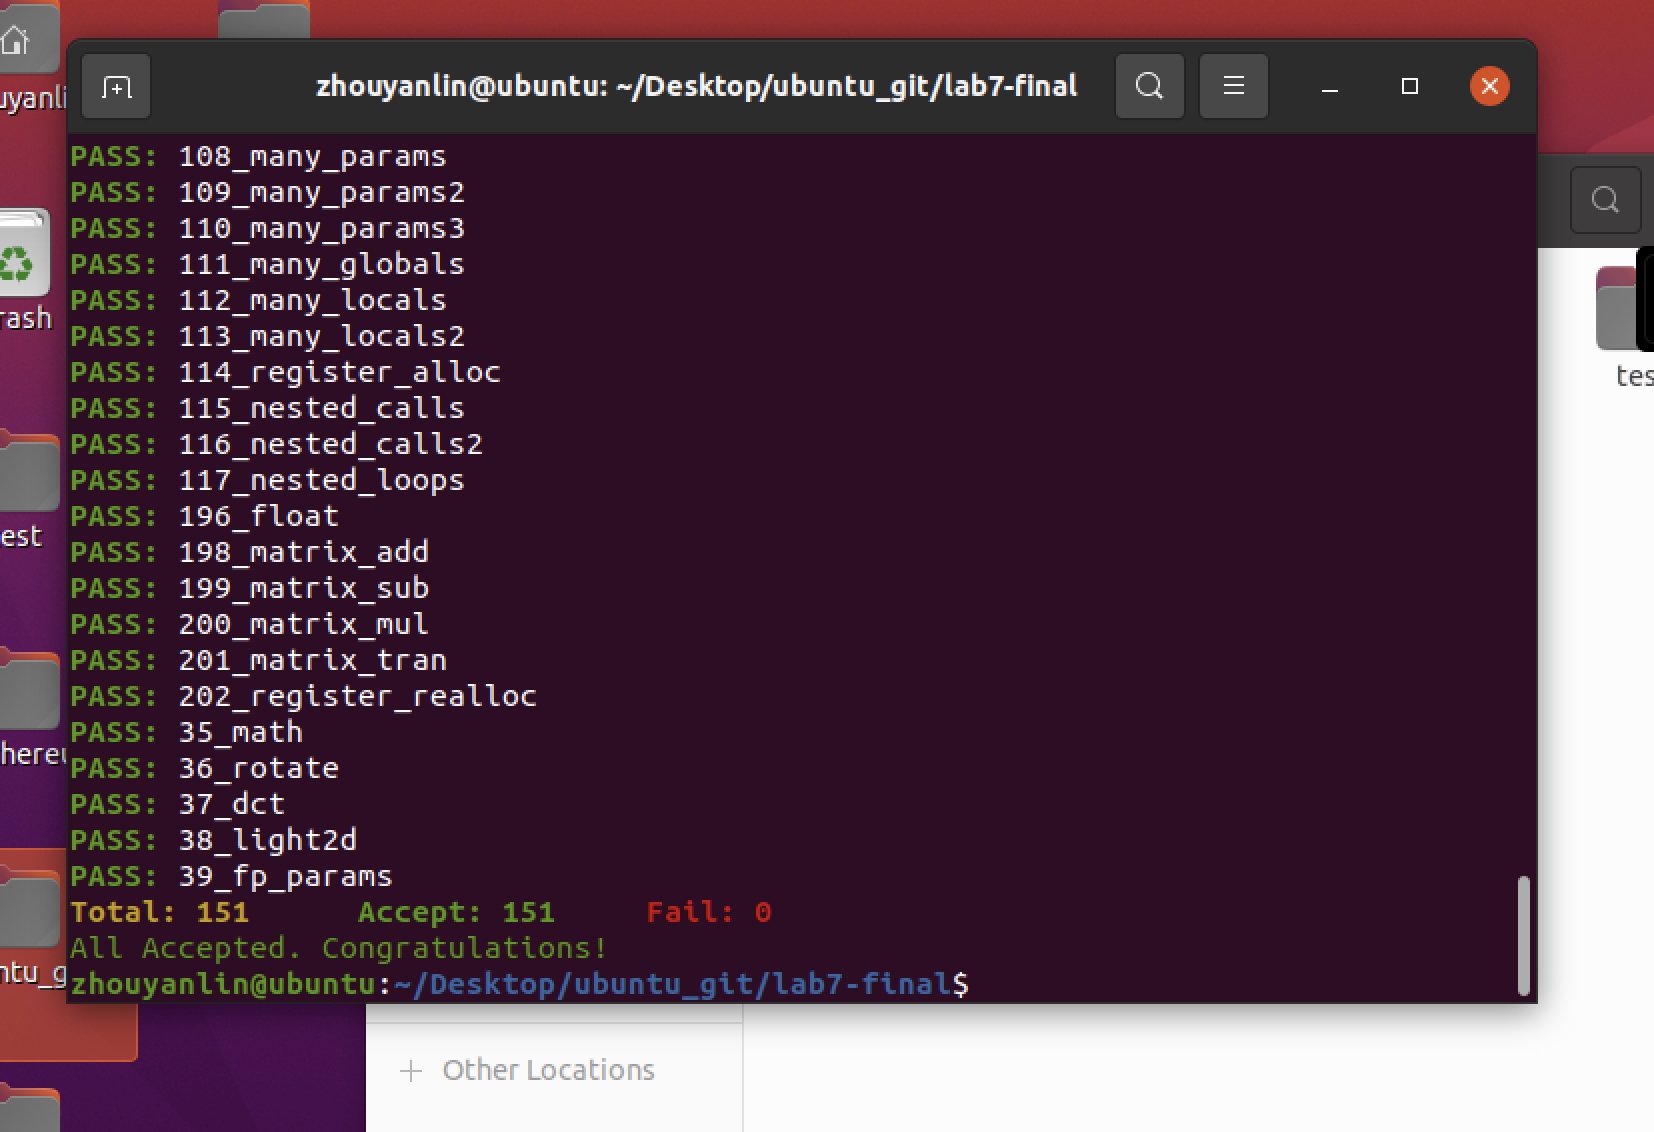
\includegraphics[scale=0.5]{1.png}
    \caption{编译器运行结果}
    \label{fig:1}
\end{figure}




% 目标代码生成结束
%----------------------------------------------------------------









%----------------------------------------------------------------
% 代码优化开始
\newpage

\section{代码优化}
\subsection{思想简介}
\subsubsection{Mem2Reg}
Mem2Reg 是 LLVM 采用的 SSA 转换算法。如果使用 LLVM 作为后端,编译器前端在生成 LLVM IR时可以先生成\fbox{alloca/load/store}这样借助内存存储局部变量值的 SSA 形式(即可以先不生成$\varphi$函数)。在 LLVM 拿到前端生成的代码后,Mem2Reg 会将这些指令删除,并插入合适的$\varphi$ 函数。

例如下面这段代码:
\begin{lstlisting}[title = 样例函数, language = c++]
int main() {
    int x, cond = 1;
    if (cond > 0)
        x = 1;
    else
        x = -1;
    return x;
}
\end{lstlisting}

前端生成的代码:
\begin{lstlisting}[title = 中间代码]
define dso_local i32 @main() {
    %1 = alloca i32
    %2 = alloca i32
    store i32 1, i32* %1
    %3 = load i32, i32* %1
    %4 = icmp sgt i32 %3, 0
    br i1 %4, label %5, label %8

5:
    store i32 1, i32* %2
    br label %6

6:
    %7 = load i32, i32* %2
    ret i32 %7

8:
    %9 = sub i32 0, 1
    store i32 %9, i32* %2
    br label %6
}
\end{lstlisting}

Mem2Reg 转换后的代码:
\begin{lstlisting}[title = 转换]
define dso_local i32 @main() {
    %1 = icmp sgt i32 1, 0
    br i1 %1, label %2, label %5

2:
    br label %3

3:
    %4 = phi i32 [ 1, %2 ], [ %6, %5 ]
    ret i32 %4

5:
    %6 = sub i32 0, 1
    br label %3
}
\end{lstlisting}
\subsubsection{图着色寄存器分配}
如果寄存器分配问题被抽象成图着色问题,那么图中的每个节点代表某个变量的活跃期或生存期(Live range)。活跃期定义是从变量第一次被定义(赋值)开始,到它下一次被赋值前的最后一次被使用为止。两个节点之间的边表示这两个变量活跃期因为生命期(lifetime)重叠导致互相冲突或干涉。一般说来,如果两个变量在函数的某一点是同时活跃(live)的,它们就相互冲突,不能占有同一个寄存器。

基于着色图分配寄存器的过程就是将不同颜色对应不同物理寄存器,颜色数量k对应物理寄存器数量。通过图着色方法可以为变量分配寄存器而不产生冲突。当然,寄存器分配比较复杂,不仅仅是图着色的问题。比如,当物理寄存器数目不足以分配给所有变量时,就必须将某些变量溢出到内存中,即spill。最小化溢出代价的问题,也是一个NP-complete问题。

图着色寄存器分配也是对线性寄存器分配的一个优化。
\subsection{个人贡献}
由于代码优化部分主要是由我的队友负责,我在这部分是与队友讨论思想和算法,然后确定好一个比较高效的实现方式后去完成。





% 代码优化结束
%----------------------------------------------------------------









%----------------------------------------------------------------
% \newpage
% \section{概述}
% %——————————————————————————————————————
% \subsection{第一节}
% 如图\ref{fig:1}所示
% \begin{figure}[H]
%     \centering
%     \includegraphics[scale=0.3]{NKU.png}
%     \caption{Caption}
%     \label{fig:1}
% \end{figure}

% 表
% \begin{table}[!htbp]
%   \centering
%   \begin{tabular}{ccccccccccc}
%   \toprule  
%   N/n$\backslash$Algo& naive-conv& naive-pool& omp-conv& omp-pool\\
%   \midrule
%   64/2& 0.0167& 0.01255& 0.04142& 0.03799\\
%   64/4& 0.03599&0.0394& 0.0458& 0.0421\\
%   \bottomrule
%   \end{tabular}
%   \caption{性能测试结果(4线程)(单位:ms)}
% \end{table}

% 带单元格表格
% \begin{table}[!htbp]
%   \centering
%   \begin{tabular}{|c|c|c|c|c|c|c|}
%   \hline
%   \multicolumn{2}{|c|}{ \multirow{2}*{$Cost$} }& \multicolumn{5}{c|}{To}\\
%   \cline{3-7}
%   \multicolumn{2}{|c|}{}&$A$&$B$&$C$&$D$&$E$\\
%   \hline
%   \multirow{3}*{From}&$B$&7&0&1&3&8\\
%   \cline{2-7}
%   &$C$&8&1&0&2&7\\
%   \cline{2-7}
%   &$D$&8&3&2&0&5\\
%   \hline
%   \end{tabular}
%   \caption{结点C距离向量表(无毒性逆转)}
% \end{table}

% %——————————————————————————————————————
% \subsection{第二节}
% 伪代码

% \begin{breakablealgorithm} 
%   \caption{初始化obj文件信息——对应MeshSimplify类中readfile函数,Face类calMatrix函数} 
%   \begin{algorithmic}[1] %每行显示行号  
%       \Require obj文件,顶点、边、面列表
%       \Ensure 是否读取成功
%       \Function {calMatrix}{$Face$}  
%               \State $normal \gets e1×e2$  
%               \State $normal \gets normal/normal.length$
%               \State $temp[] \gets {normal.x, normal.y, normal.z, normal· Face.v1}$
%               \State $Matrix[i][j]=temp[i] * temp[j]$ 
%               \State \Return{$Matrix$}  
%       \EndFunction
%       \State 根据obj的v和f区分点面信息,读取并加入列表
%       \State $scale \gets $记录点坐标中距离原点最远的分量,以便后续OpenGL进行显示
%       \State $ori \gets $记录中心点,便于OpenGL显示在中心位置,避免有的obj偏移原点较多
%       \State 根据三角面片信息,计算一个面的三条边
%       \State 计算每个面的矩阵$\gets calMatrix$
%       \State 将每个面的矩阵加到各点,由点维护\\
%       \Return True
%   \end{algorithmic}  
% \end{breakablealgorithm}

% 代码
% \begin{lstlisting}[title=逐列访问平凡算法,frame=trbl,language={C++}]
%   void ord()   
%   {
%       double head,tail,freq,head1,tail1,timess=0; // timers
%       init(N);
%       QueryPerformanceFrequency((LARGE_INTEGER *)&freq );
%       QueryPerformanceCounter((LARGE_INTEGER *)&head);
%       for (int i=0; i<NN; i++)
%           for (int j=0; j<NN; j++)
%               col_sum[i] += (b[j][i]*a[j]);
%       QueryPerformanceCounter ((LARGE_INTEGER *)& tail) ;
%       cout << "\nordCol:" <<(tail-head)*1000.0 / freq<< "ms" << endl;
%   }
% \end{lstlisting}


% %——————————————————————————————————————
% \subsection{第三节}

% 参考文献\cite{adams1995hitchhiker}\cite{shin2016deep}
    
% 多行公式
% \begin{align}
%   a+b = a + b \\
%   \frac{a+b}{a-b}
% \end{align}

% 行内公式:$\sum^N_{i=1}$

% \textbf{超链接}  \href{http://youtube.com/}{YouTube}

% 带标号枚举
% \begin{enumerate}
%   \item 1
%   \item 2
% \end{enumerate}

% 不带标号枚举
% \begin{itemize}
%   \item 1
%   \item 2
% \end{itemize}

% \xiaosi{切换字体大小}

%----------------------------------------------------------------
\newpage
\section{总结与展望}
\subsection{学期总结}
在本学期的编译原理实验中,从总体上来说,我们设计实现了一个较为完整的拥有前端和后端、能够生成可执行文件并且检测能够程序运行结果的简单编译器,该编译器的最终设计目的得到了实现。


我们的编译器能够识别标准SysY所支持的绝大部分词法符号,支持了变量的定义、数组的定义、函数的声明、各类表达式语句、if-else 条件语句和 while循环语句,在语义动作上可以生成相应语句动作的四也可以对相应的错误进行检测,从而实现了编译前端。

在中间代码部分我们可以成功将其生成LLVM体系下的中间代码,并在对应实验中取得了满分的成绩,最后对于目标代码我们不仅通过了本学期所有的基本和提升要求的151个样例,并对寄存器的分配和SSA语言进行了优化,整体下来获益匪浅,我们高质量完成了一个相对工程量大的项目,这也是属于程序员的浪漫。

\subsection{未来展望}
最后这次实验做完也已经准备开启大三下,其实大学生活也剩的不多了。大学生活是对一个人整体的考验,正是如此,才造就了今天的我。现在也在人生的岔路口中,不论将来是出国还是保研,我都很感谢编译原理这门课程对我的磨练,希望自己在今后的人生中可以得到更好的发展,\fbox{万事胜意、心想事成、未来可期}。

\newpage
\section*{致谢}

\kaishu{行文至此,落笔为终。人生已二十载,岁月匆匆。目之所及,尽是回忆;心之所想,皆是过往。值此之际,亦道不尽心中谢意。}


独学而无友,则孤陋而寡闻。我要感谢王刚老师在学习上给予的帮助,在此表示诚挚的谢意!桂花同载酒,不负少年游。更要感谢一路陪伴的朋友们,让我可以分享快乐与失意,感受温暖和力量,愿我们都前程似锦。 

父母之爱子,则为之计深远。借此机会,特别感谢我的父母和家人。在我二十载的求学路上,是你们的默默付出与支持,激励着我砥砺前行。灿灿萱草花,罗生北堂下。南风吹其心,摇摇为谁吐?春晖寸草,难以回报。愿你们平安康乐,岁月无恙。 

欲谢之人众多,然纸短情长,未能提及者,吾深表歉意。诸君之恩,吾没齿难忘。梧高凤必至,花香蝶自来。人终向前走,花自向阳开。
%----------------------------------------------------------------
% \newpage
% \bibliographystyle{plain}
% \bibliography{references} 
%---------------------------------------------------------------
\newpage
% \vspace*{300pt}
\bibliographystyle{plain}
\bibliography{references} 
\end{document}
